\documentclass{cmspaper}
\usepackage{amsmath}
\usepackage{epsfig}
\begin{document}

%==============================================================================
% title page for few authors

\begin{titlepage}

% select one of the following and type in the proper number:
%  \internalnote{2009/000}
%  \conferencereport{2005/000}
   \date{\today}

%  \title{A study of isolation for SUSY low-$p_T$ leptons}
 \title{Study of isolation properties of SUSY low-$p_T$ leptons.}

  \begin{Authlist}
    Z.~Hatherell\Aref{a}, G.~Karapostoli\Aref{a}, M.~Pioppi\Aref{a, b},\\
 A.~Savin\Aref{c},
    A.~Sparrow\Aref{a}, M.~Weinberg\Aref{c}
       \Instfoot{ic}{a) Imperial College London, United Kingdom}
       \Instfoot{perugia}{b) INFN e Dipartimento di Fisica, Perugia, Italy}
       \Instfoot{wisconsin}{c) University of Wisconsin, Madison, United States}
  \end{Authlist}

  \begin{abstract}
    Events with leptons in the final state will play a significant role in SUSY searches at initial
    LHC luminosities. The energy spectra of the leptons is expected to be soft, especially in models
    where the mass difference between the initial SUSY particle and the lightest SUSY particle (LSP)
    is small. Optimization of isolation cuts for electrons in the transverse momentum range
    $5 < p_T < 30~{\rm GeV}$ and for muons in the range $3 < p_T < 30~{\rm GeV}$ is discussed. The
    results are presented in terms of SUSY lepton reconstruction efficiency and rejection of fake
    leptons and leptons from heavy quark decays. Lepton selections for single- and double-lepton
    SUSY final states are proposed.
  \end{abstract}

% if needed, use the following:
%\conference{Presented at {\it Physics Rumours}, Coconut Island, April 1, 2005}
%\submitted{Submitted to {\it Physics Rumours}}
%\note{Preliminary version}

\end{titlepage}

\setcounter{page}{2}%JPP

%==============================================================================
% title page for many authors
%
%\begin{titlepage}
%  \internalnote{2005/000}
%  \title{CMS Technical Note Template}
%
%  \begin{Authlist}
%    A.~Author\Iref{cern}, B.~Author\Iref{cern}, C.~Author\IAref{cern}{a},
%    D.~Author\IIref{cern}{ieph}, E.~Author\IIAref{cern}{ieph}{b},
%    F.~Author\Iref{ieph}
%  \end{Authlist}
%
%  \Instfoot{cern}{CERN, Geneva, Switzerland}
%  \Instfoot{ieph}{Institute of Experimental Physics, Hepcity, Wonderland}
%  \Anotfoot{a}{On leave from prison}
%  \Anotfoot{b}{Now at the Moon}
%
%  \begin{abstract}
%    This is a template of a CMS paper, written in LaTeX,
%    processed with {\it cmspaper.sty} style.
%    It is based on the {\it cernart.sty} and {\it articlet.sty} styles.
%    There are two versions of the title page.
%    The current one is designed for many authors.
%    The one on the previous page is for few authors.
%    Just delete the one which you do not need.
%  \end{abstract}
%
%\end{titlepage}
%
%==============================================================================

\section{Introduction}
\label{sec:intro}

Events with leptons in the final state will play a significant role in SUSY searches already at
initial LHC luminosities. They complement the fully-hadronic searches, providing cleaner signatures
than those based just on jets and missing energy.

SUSY models predict significant lepton production from decay of sparticles. The primary sources of
leptons are expected to be:

\begin{align*}
   \tilde{\chi}_2^0     \rightarrow l^{\pm} + \tilde{l}^{\mp} \\
   \tilde{\chi}_1^{\pm} \rightarrow l^{\pm} + \tilde{\nu}_l   \\
   \tilde{l}^{\pm}      \rightarrow l^{\pm} + \tilde{\chi}_1^0
\end{align*}

The $p_T$ spectrum of the resulting leptons depends strongly on the mass difference between the
initial and final SUSY particles. For the cases in which the two SUSY particles are more nearly
mass-degenerate, the lepton $p_T$ spectrum is expected to be soft, and therefore a high
lepton-reconstruction efficiency and background rejection at low transverse momentum is required.

The standard lepton-isolation recommendations at CMS proposed by the V + Jets Cross-PAG~\cite{vjets}
have been shown to work well for lepton-$p_T$ above $\sim 30$ GeV/$c$. For lower-$p_T$ leptons,
however, these cuts can have a much more pronounced impact on the efficiency. For this reason, it is
natural to look at separate optimization of the isolation requirements for soft leptons.

\section{Lepton reconstruction and isolation requirements}
\label{sec:lepRecoIsoReq}
The analysis was performed within the SUSY PAT framework~\cite{susypat}. From the PAT data format,
reduced ntuples were produced using the procedure described elsewhere~\cite{ICNT}. The data samples are
summarized in Table~\ref{tab:samples}.

\begin{table}[htbp]
   \centering
\begin{tabular}{|c|c|c|}
\hline
Sample & N MC events & $\sigma$ (pb) \\
\hline
SUSY (LM1) & 104800 & 16.06 \\
\hline
QCD (Pythia) & 27267325 & 1.568 $\times 10^9$ \\
\hline
\end{tabular}
   \caption{\small{MC samples used for the isolation study.}\label{tab:samples}}
\end{table}


For the purposes of the lepton isolation performace study, we have developed a lepton classification tool based on the Monte Carlo (MC) truth information. Reconstructed electrons and muons are matched to generator level leptons ($e$ or $\mu$'s), and split into the following categories, according to the MC mother of the generated particle: i) ``Prompt'' leptons, are identified as the ones originated by the decay of a SUSY particle, a $W/Z$ or a $\tau$. ii) ``Heavy-flavor'' leptons, are coming from the hadronic decays of heavy-flavor quarks ($b/c$ decays). iii) ``Fake'' leptons are typically identified as reconstructed leptons faked by a jet. In the case of muons, the latter category includes in-flight decays of $\pi/K$-mesons, as well as jet punch-through.


%At generator level, ``prompt'' leptons are defined  as those coming directly from a SUSY decay or from
%a $W$, $Z$ or $\tau$ coming from a SUSY decay, and ``Heavy Flavor (HF)'' leptons are all other leptons
%appearing during the hadronization stage. Radiative leptons from prompt leptons were not considered
%to avoid double counting.

Matching between generated and reconstructed leptons was performed using a
cone in ($\eta, \phi$) phase space. The distance between generated and reconstructed leptons,
$\Delta R = \sqrt{(\Delta \eta)^2 + (\Delta \phi)^2}$, was required to be less then 0.5, and the
closest generated lepton was associated with the corresponding reconstructed candidate. If no
generated lepton was found within the $\Delta R$ cone the reconstructed lepton was considered to be
a ``fake''.

The leptons were reconstructed at detector level and passed identification
procedure~\cite{elecid,muonid}. Electrons that satisfied RobustLoose and muons that satisfied
GlobalTight identification requirements were selected. Generated and reconstructed electrons were
required to have $p_T > 5~{\rm GeV}$ and $|\eta| < 2.5$, muons, $p_T > 3~{\rm GeV}$ and
$|\eta| < 2.1$. In order to reduce contribution form the HF and fake leptons, additional requirements on the lepton qualiity were applied:
\begin{itemize}
\item Transverse impact parameter corrected for the beam spot $<$ 2 mm
\item Normalized global $\chi^2 <$ 10 (only for muons)
\item Number of hits in the tracker track $>$ 11 (only for muons)
\end{itemize}

Lepton reconstruction efficiency, defined as a ratio of the number of reconstructed and matched
leptons to the total number of generated leptons, was estimated using prompt leptons from the SUSY
LM1 sample. The efficiency is presented in Fig.~\ref{fig:genPt_recoEff_prompt} for (a) electrons and
(b) muons as a function of generated lepton $p_T$. The efficiency decreases with
decreasing lepton $p_T$, and corresponds to $\sim 60\%$ in the lowest $p_T$ bins considered in this
analysis.

\begin{figure}[htbp]
   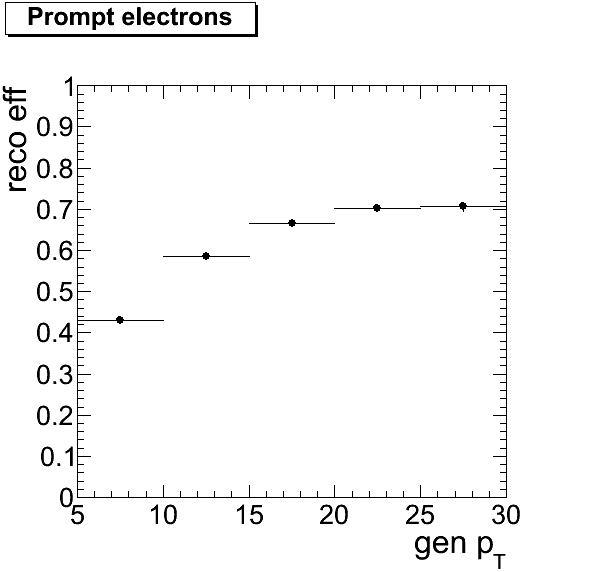
\includegraphics[width = 0.49\textwidth]{pictures/genPt_recoEff_prompt/genPt_recoEff_elec_prompt.png}
   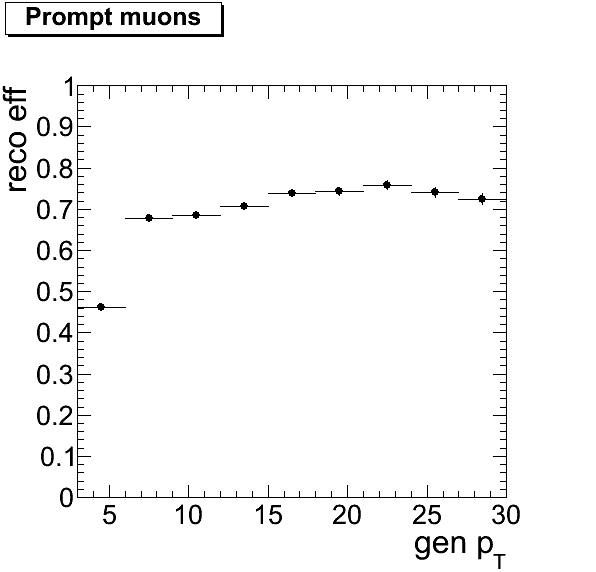
\includegraphics[width = 0.49\textwidth]{pictures/genPt_recoEff_prompt/genPt_recoEff_muon_prompt.png}
   \caption{\small{Reconstruction efficiency for (a) prompt electrons and (b) prompt muons as a function of
      generated lepton $p_T$.}
   \label{fig:genPt_recoEff_prompt}}
\end{figure}

Isolation properties of the reconstructed leptons were studied using
%Prompt and HF reconstructed leptons can be separated by applying additional isolation
%requirements, which are based on the following isolation variables:
 following isolation variables:

\begin{align*}
   \textrm{iso}_{\textrm{abs}}^{\textrm{track}} & = \sum_{\Delta R < 0.3} p_T^{\textrm{track}} \\
   \textrm{iso}_{\textrm{abs}}^{\textrm{ECAL}}  & = \sum_{\Delta R < 0.3} E_T^{\textrm{ECAL}}  \\
   \textrm{iso}_{\textrm{abs}}^{\textrm{HCAL}}  & = \sum_{\Delta R < 0.3} E_T^{\textrm{HCAL}}  \\
   \textrm{iso}_{\textrm{abs}}^{\textrm{comb}}  & = \sum_{\Delta R < 0.3}\left(p_T^{\textrm{track}} + E_T^{\textrm{ECAL} + \textrm{HCAL}}\right) \\
%   \textrm{iso}_{\textrm{rel}}^{\textrm{track}} & = \frac{\sum_{\Delta R < 0.3} p_T^{\textrm{track}}}{p_T^l} \\
%   \textrm{iso}_{\textrm{rel}}^{\textrm{ECAL}}  & = \frac{\sum_{\Delta R < 0.3} E_T^{\textrm{ECAL}}}{p_T^l}  \\
%   \textrm{iso}_{\textrm{rel}}^{\textrm{HCAL}}  & = \frac{\sum_{\Delta R < 0.3} E_T^{\textrm{HCAL}}}{p_T^l}  \\
%   \textrm{iso}_{\textrm{rel}}^{\textrm{comb}}  & = \frac{\sum_{\Delta R < 0.3}\left(p_T^{\textrm{track}} + E_T^{\textrm{ECAL} + \textrm{HCAL}}\right)}{p_T^l}
\end{align*}

where $\sum_{\Delta R < 0.3} p_T^{\textrm{track}}$ is the sum of the transverse momenta of the
tracks in a cone ($\Delta R < 0.3$) around the lepton direction.
$\sum_{\Delta R < 0.3} E_T^{\textrm{ECAL}}$ and $\sum_{\Delta R < 0.3} E_T^{\textrm{HCAL}}$ are the
sums of the transverse energy measured in a cone ($\Delta R < 0.3$) around the lepton direction in the
electromagnetic and hadronic calorimeter respectively. Relative isolation was defined as a ratio of the
absolute isolation to reconstructed transverse momentum, $p_T$, of the examined lepton.

A scatter plot of combined relative isolation as a function of reconstructed lepton $p_T$ is presented in
Fig.~\ref{fig:recoPt_combRelIso_prompt} for prompt, HF and fake leptons respectively. The V +
Jets Cross-PAG recommended cut of 0.1 is also shown. At low $p_T$ values the cut rejects a significant
fraction of signal events; therefore, additional optimization of the isolation procedure is
needed. Since the isolation depends on the lepton transverse momentum, the
optimization is done in multiple bins of lepton $p_T$.
%. Electrons are divided into five  bins
% of 5 GeV width
%starting from 5 GeV (
Five bins of 5 GeV width: 5 -- 10 GeV, 10 -- 15 GeV, ..., 25 -- 30 GeV for electrons
% ) and Muons are divided into 9 bins of
%3 GeV width starting from
and nine bins of 3 GeV width: 3 -- 6 GeV, 6 -- 9 GeV, ..., 27 -- 30 GeV for muons.
%In order to study the
%isolation behavior of very low energy muons a smaller $p_T$ bin width was adopted. In both cases,
The lower limits on the $p_T$ ranges represent the softest leptons that can be reconstructed within
the PAT framework and bin width is choosen based on energy resolution.

\begin{figure}[htbp]
   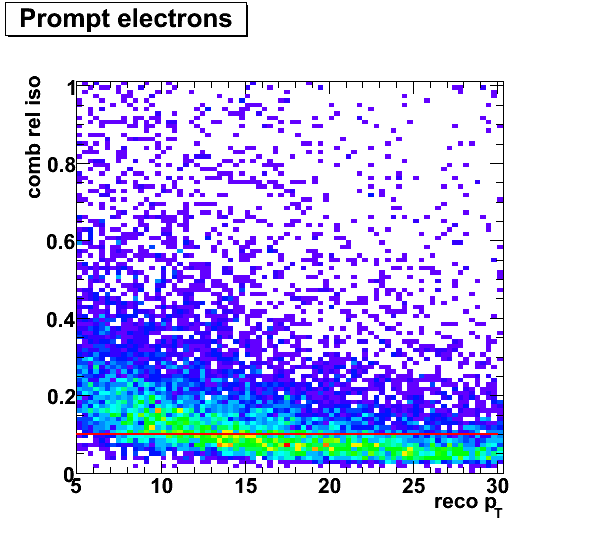
\includegraphics[width = 0.49\textwidth]{pictures/recoPt_relIso/combIso_elec_prompt.png}
   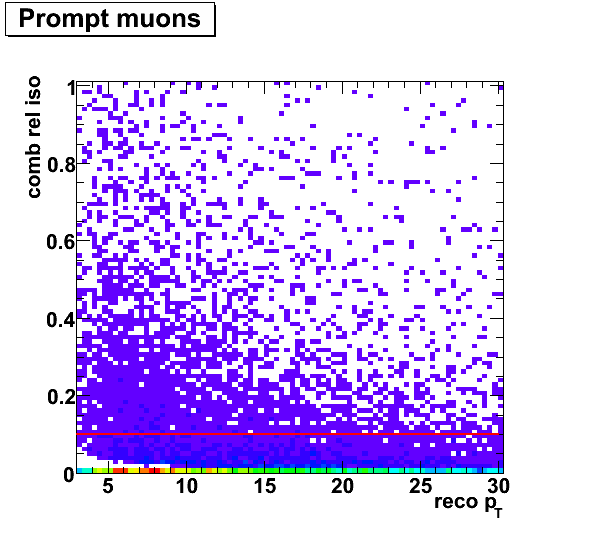
\includegraphics[width = 0.49\textwidth]{pictures/recoPt_relIso/combIso_muon_prompt.png} \\
   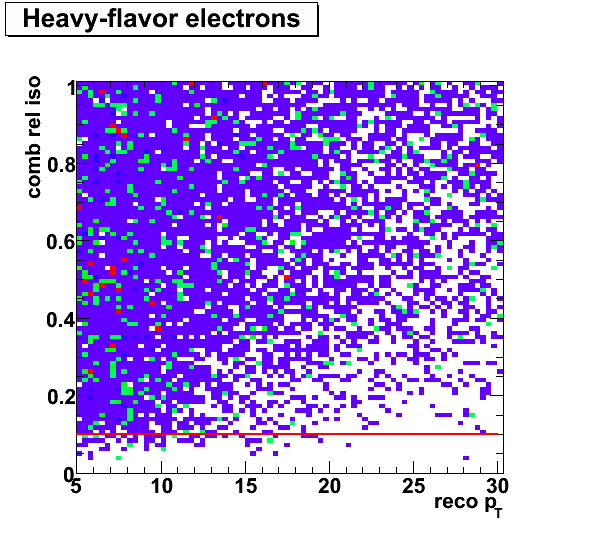
\includegraphics[width = 0.49\textwidth]{pictures/recoPt_relIso/combIso_elec_nonPrompt.png}
   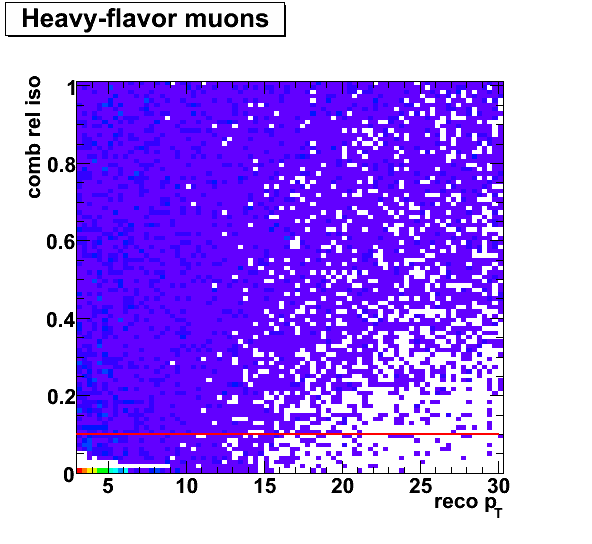
\includegraphics[width = 0.49\textwidth]{pictures/recoPt_relIso/combIso_muon_nonPrompt.png}\\
   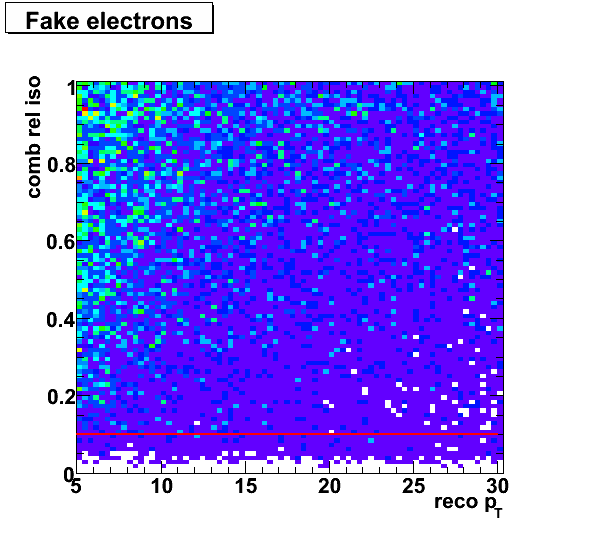
\includegraphics[width = 0.49\textwidth]{pictures/recoPt_relIso/combIso_elec_fake.png}
   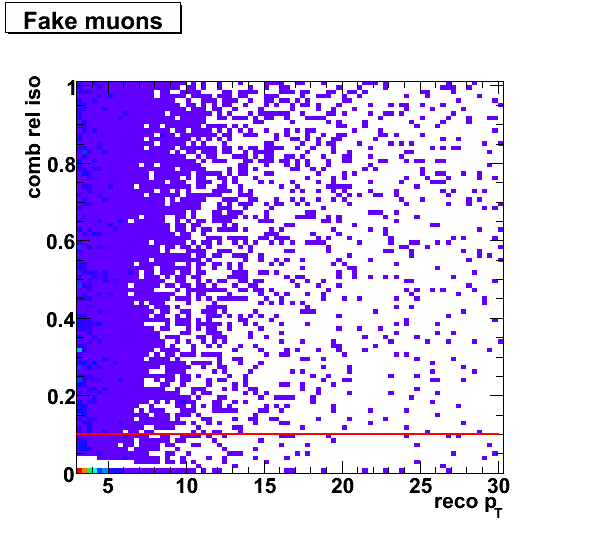
\includegraphics[width = 0.49\textwidth]{pictures/recoPt_relIso/combIso_muon_fake.png}
   \caption{\small{Combined relative isolation as a function of reconstructed $p_T$ for prompt
(top), HF (middle) and fake (bottom) leptons. Electrons are shown on the left while muons are on the right.}
   \label{fig:recoPt_combRelIso_prompt}}
\end{figure}

%\begin{figure}[htbp]
%   \caption{\small{Combined relative isolation as a function of reconstructed $p_T$ for (a) hadronic
%      electrons and (b) hadronic muons}
%   \label{fig:recoPt_combRelIso_nonPrompt}}
%\end{figure}

%\begin{figure}[htbp]
%   \caption{\small{Combined relative isolation as a function of reconstructed $p_T$ for (a) fake
%      electrons and (b) fake muons}
%   \label{fig:recoPt_combRelIso_fake}}
%\end{figure}

%\clearpage

\section{Optimization of isolation requirements for low-$p_T$ leptons}
\label{sec:softLepIsoOpt}
%As stated in Sec.~\ref{sec:intro}, the goal of this work is
The optimization of the isolation for
leptons originating from SUSY processes requires
%. For this reason,
an additional cut $HT > 300 {\rm GeV}$, where
$HT =\left(\sum_{\textrm{jets}}p_T + \sum_{\textrm{lep}}p_T \right) $, and the sums run over all the reconstructed leptons and all the reconstructed
hadronic jets with a tranverse energy greater than 50 GeV.
This cut
defines an energy scale which is expected in SUSY production.
%motivated by the requirement that we improve soft lepton isolation at the energy scale at which
%SUSY processes are expected.

The optimization procedure was based on a comparison of signal efficiency and background rejection.
Efficiency as a function of isolation cut, $\textrm{eff}(x)$, was defined as the ratio of
reconstructed leptons with isolation $< x$ to all reconstructed leptons. Rejection as a function of
isolation cut, $\textrm{rej}(x)$, was defined as the ratio of reconstructed leptons
with isolation $> x$ to all reconstructed leptons, i.e. for all cut values $x$,
$\textrm{rej}(x) = 1 - \textrm{eff}(x)$. Figure~\ref{fig:Elec_PtCut0_PtCut1}
shows prompt lepton efficiency as a function of background lepton
rejection for each isolation variable.

\begin{figure}[htbp]
\begin{center}
   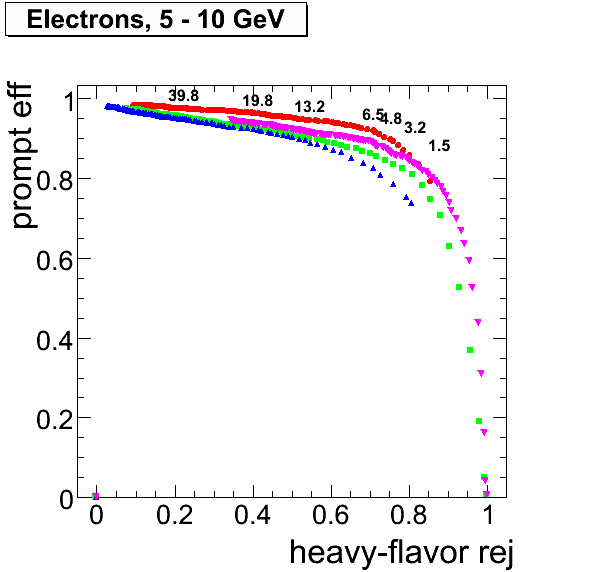
\includegraphics[width = 0.49\textwidth]{pictures/bkgdRej_sigEff/elec_nonPrompt_ptCut0_ptCut1.png}
   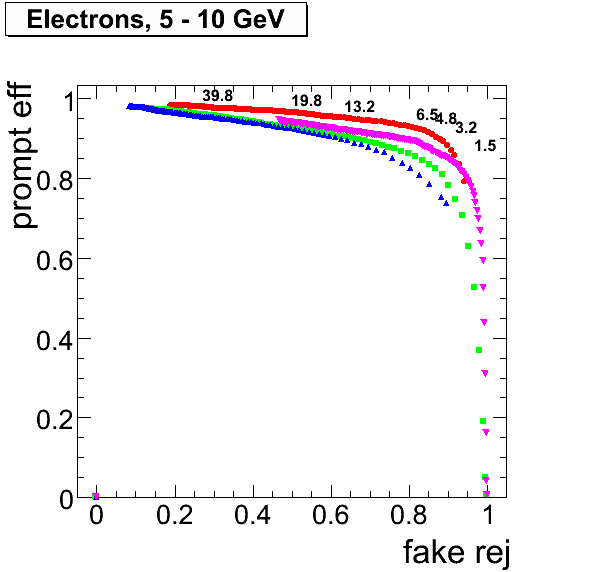
\includegraphics[width = 0.49\textwidth]{pictures/bkgdRej_sigEff/elec_fake_ptCut0_ptCut1.png} \\
   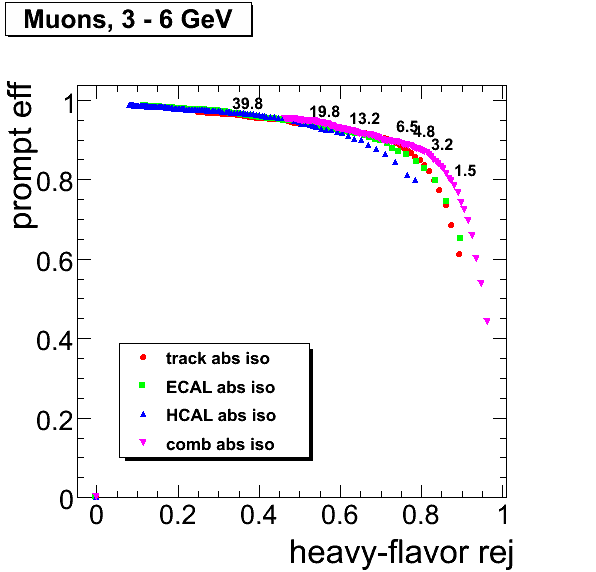
\includegraphics[width = 0.49\textwidth]{pictures/bkgdRej_sigEff/muon_nonPrompt_ptCut0_ptCut1.png}
   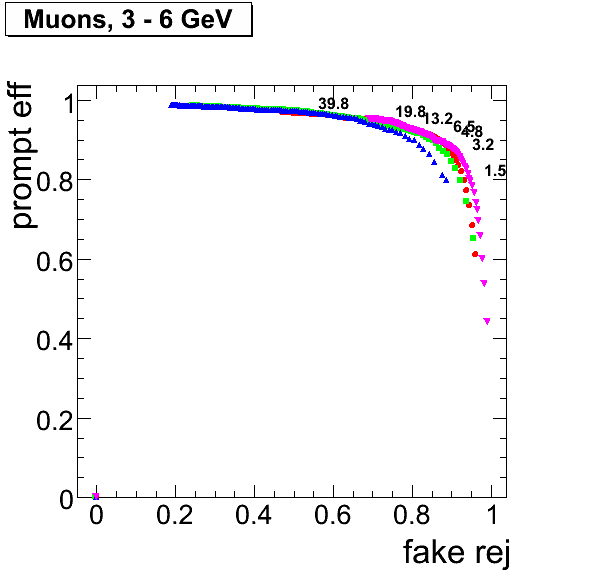
\includegraphics[width = 0.49\textwidth]{pictures/bkgdRej_sigEff/muon_fake_ptCut0_ptCut1.png}
   \caption{\small{Prompt leptons efficiency  with respect to background rejection for HF (left) and  fake
      leptons (right) in $p_T$ region from 5 to 10 GeV for electrons (top) and
       in $p_T$ region from 3 to 6 GeV for muons (bottom).
      Each point on the graph represents a different cut on absolute
      isolation calculated from the tracker (first curve), the ECAL (second curve) or the HCAL
      (third curve). }
% 	Electrons are shown on the top while muons are on the bottom. }
   \label{fig:Elec_PtCut0_PtCut1}}
\end{center}
\end{figure}

For both electrons and muons, tracker isolation demonstrates
greater discriminating power than ECAL or HCAL isolation.
%, as expected for low $p_T$ leptons.
Additionally in the LHC startup scenario,
the low $p_T$ tracks (which mainly contribute to the soft lepton isolation)
are expected to be more reliable
than the low $p_T$ energy deposits in the calorimeters, therefore
%For these reasons, we start by optimizing the tracker isolation.
only the tracker isolation is considered in the first step of the
optimization.
%Only after finding the optimal tracker
%isolation cut will we examine ECAL and HCAL isolation. Because each SUSY analysis may require a
%different prompt lepton efficiency and purity, four different isolation cuts are defined:

Since signal to background conditions differ depending on SUSY analysis four optimization
approaches were considered:

\begin{itemize}
\item {\bf PureHF} \\
%Cut with highest prompt efficiency for which $\textrm{rej}_{\textrm{HF}} \geq 0.9$
Highest cut on isolation at which $\textrm{rej}_{\textrm{HF}} \geq 0.9$
\item {\bf PureFake} \\
%Cut with highest prompt efficiency for which $\textrm{rej}_{\textrm{fake}} \geq 0.9$
Highest cut on isolation at which $\textrm{rej}_{\textrm{fake}} \geq 0.9$
\item {\bf Optimal}\\
Minimizes $x = \sqrt{(1 - \textrm{eff})^2 + (1 - \textrm{rej})^2}$
\item {\bf Efficient} \\
%Cut with highest background rejection for which $\textrm{eff}_{\textrm{prompt}} \geq 0.9$
Lowest cut on isolation at which $\textrm{eff}_{\textrm{prompt}} \geq 0.9$
\end{itemize}


\begin{figure}[htbp]
\begin{center}
   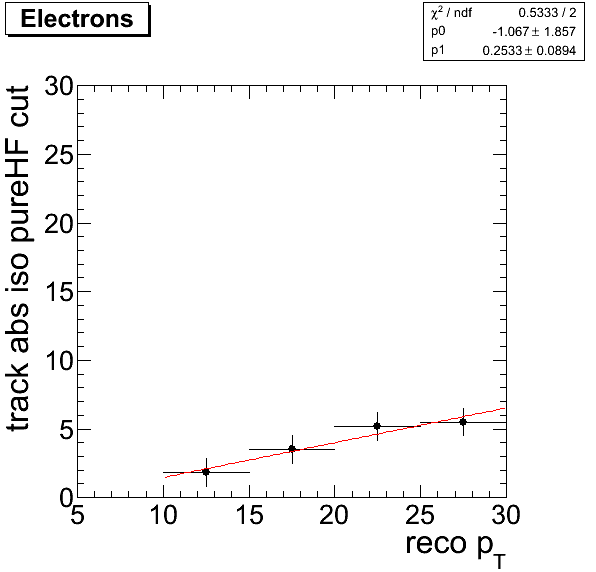
\includegraphics[width = 0.49\textwidth]{pictures/optIsoCut/trackIso_elec_pure_HF.png}
   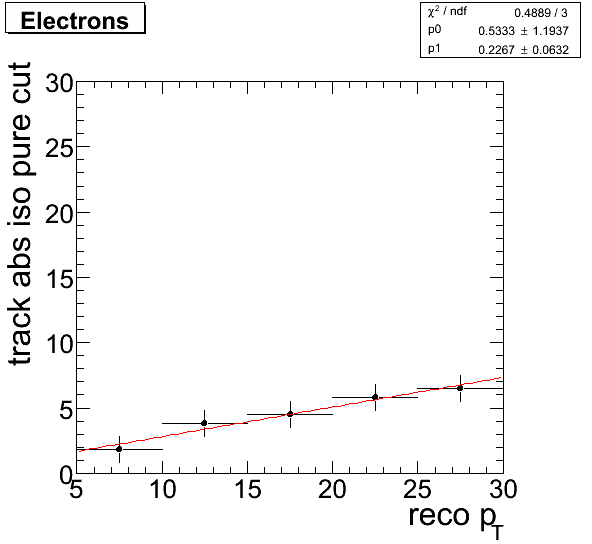
\includegraphics[width = 0.49\textwidth]{pictures/optIsoCut/trackIso_elec_pure.png}
   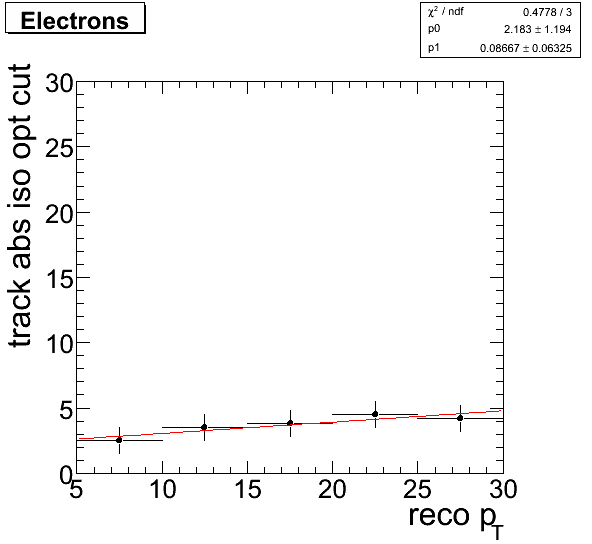
\includegraphics[width = 0.49\textwidth]{pictures/optIsoCut/trackIso_elec_opt.png}
   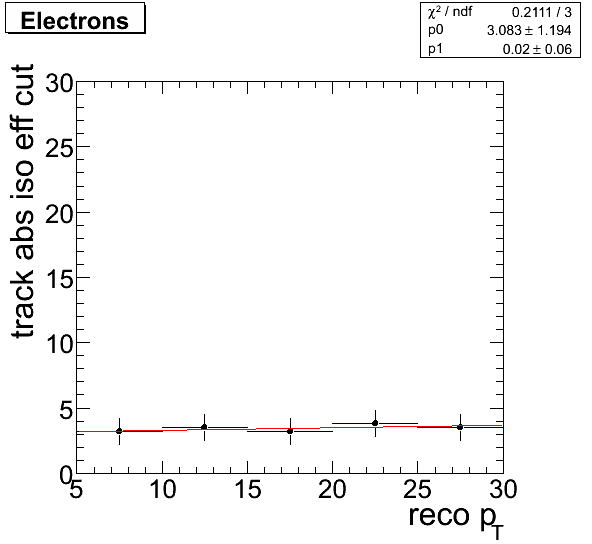
\includegraphics[width = 0.49\textwidth]{pictures/optIsoCut/trackIso_elec_eff.png}
    \caption{\small{\label{fig:optTrackIso_elec}Tracker isolation
 cut values for electrons as a function of $p_T$ for {\bf pureHF}(top left), {\bf pureFake} (top right),
	{\bf optimal} (bottom left) and {\bf efficient} (bottom right) optimization procedure. }}
\end{center}
\end{figure}

Figure~\ref{fig:optTrackIso_elec} shows the optimized cut values as a function of the electron
transverse momentum. Linear fits to the data are also shown. The lowest-$p_T$ bin for the
{\bf pureHF}  procedure is empty, since the required 0.9 rejection power can not be achieved
by using tracking information only. The {\bf pure} procedures demonstrate an increase of the
isolation cat with $p_T$ increase, the {\bf efficient} requirement allows the isolation cut
to be almost constant with $p_T$.
%Efficient and optimal procedures show a reduced dependance on the momentum and require
%a tracker isolation less than 2 and 3 GeV respectively.
%The pure$_{fake}$ cut value is linearly dependent following the expression
%$\textrm{iso}_{\textrm{abs}}^{\textrm{track}} < (0.5 GeV + 0.227 p_T)$.

\begin{figure}[htbp]
\begin{center}
   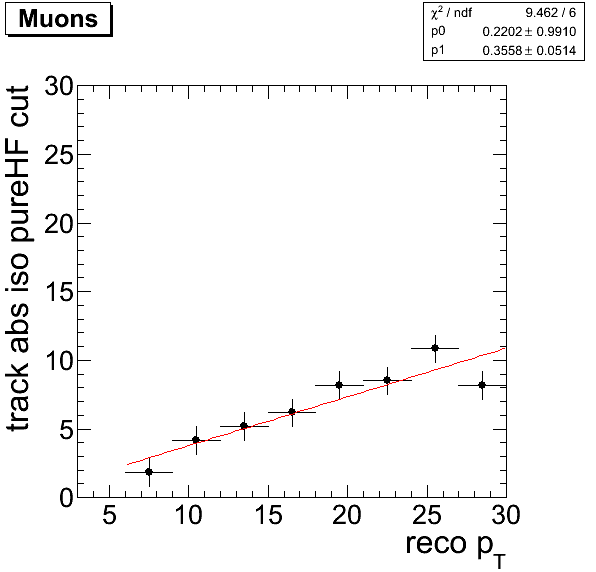
\includegraphics[width = 0.49\textwidth]{pictures/optIsoCut/trackIso_muon_pure_HF.png}
   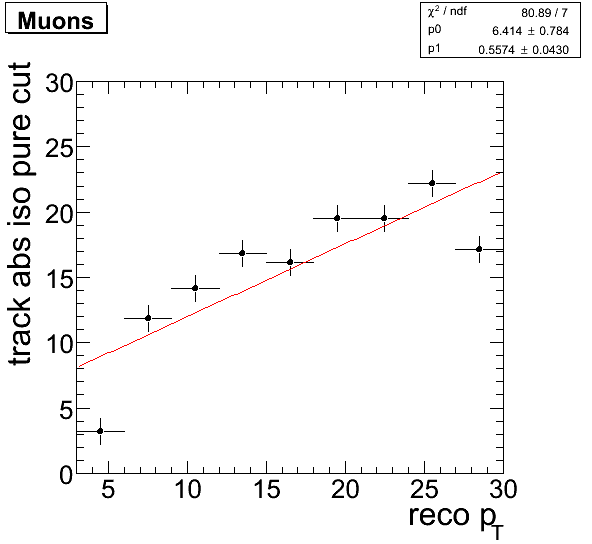
\includegraphics[width = 0.49\textwidth]{pictures/optIsoCut/trackIso_muon_pure.png}
   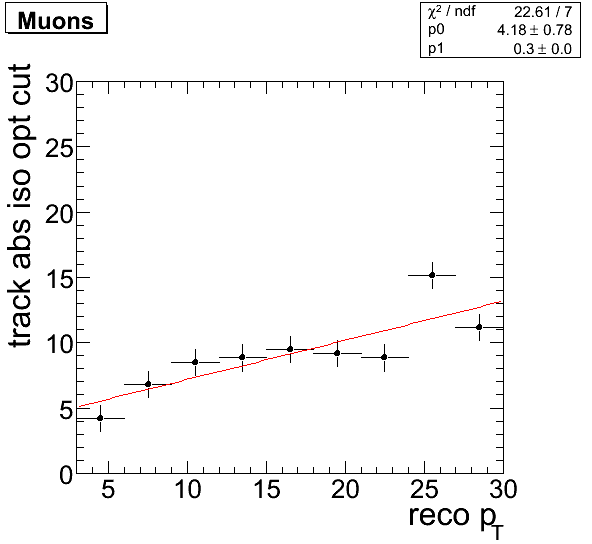
\includegraphics[width = 0.49\textwidth]{pictures/optIsoCut/trackIso_muon_opt.png}
   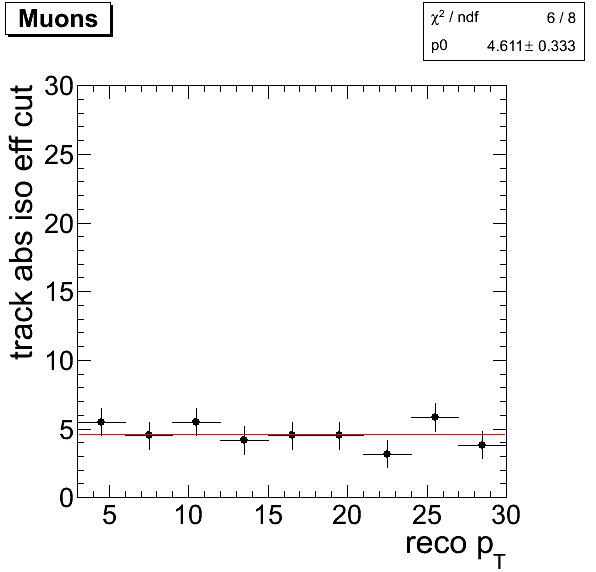
\includegraphics[width = 0.49\textwidth]{pictures/optIsoCut/trackIso_muon_eff.png}
   \caption{\small{\label{fig:optTrackIso_muon} Tracker isolation
 cut values for muons as a function of $p_T$ for {\bf pureHF} (top left), {\bf pureFake} (top right),
	{\bf optimal} (bottom left), {\bf efficient} (bottom right) optimization procedure. }}
\end{center}
\end{figure}

The optimization results for muons are presented in
Fig.~\ref{fig:optTrackIso_muon}.
% shows the optimized cut values as a function of the muon
%transverse momentum.
%Only the efficient cut values ($\textrm{iso}_{\textrm{abs}}^{\textrm{track}} < 5 GeV$) is independent
%from the momentum.
%In general the requests for muons are much less stringent than the corresponding requests
%for electrons.
The results demonstrate behaviour similar to those for muons but in general the cuts are less
stringent.

The results of the optimization procedure are summarized in App.~\ref{app:tables} and App.~\ref{app:plots_tk}.


%In App.~\ref{app:tables} for each $p_T$ bin  the optimal cut is reported with the corresponding values
%of prompt lepton  efficiency and fake and HF lepton rejection.
%Tables are provided for all the optimization procedures described above.
%In App.~\ref{app:plots_tk} for each $p_T$ bin the curves of prompt efficiency versus the background rejection are shown.

%\clearpage

\begin{table}[htbp]
   \centering
   \begin{tabular}{|c|c|c|c|c|}
      \hline
      $p_T$ range (GeV) & Optimal cut & eff & $\textrm{rej}_{HF}$ & $\textrm{rej}_{fake}$ \\
      \hline
      5 - 10 & 2.83 & 0.78 $\pm$ 0.06 & 0.835 $\pm$ 0.0016 & 0.904 $\pm$ 0.00025 \\
      \hline
      10 - 15 & 3.83 & 0.822 $\pm$ 0.056 & 0.855 $\pm$ 0.0019 & 0.911 $\pm$ 0.00031 \\
      \hline
      15 - 20 & 4.5 & 0.846 $\pm$ 0.059 & 0.883 $\pm$ 0.0022 & 0.912 $\pm$ 0.00041 \\
      \hline
      20 - 25 & 5.5 & 0.859 $\pm$ 0.065 & 0.854 $\pm$ 0.003 & 0.902 $\pm$ 0.00053 \\
      \hline
      25 - 30 & 5.83 & 0.872 $\pm$ 0.072 & 0.898 $\pm$ 0.0031 & 0.904 $\pm$ 0.00059 \\
      \hline
   \end{tabular}
   \caption{\small{Performances of the ECAL isolation for electrons when the rejection of fakes is fixed at $\geq 0.9$}\label{tab:ecal_elec_pureFake}}
\end{table}






\begin{table}[htbp]
   \centering
   \begin{tabular}{|c|c|c|c|c|}
      \hline
      $p_T$ range (GeV) & Optimal cut & eff & $\textrm{rej}_{HF}$ & $\textrm{rej}_{fake}$ \\
      \hline
      5 - 10 & 1.83 & 0.628 $\pm$ 0.069 & 0.905 $\pm$ 0.0013 & 0.955 $\pm$ 0.00017 \\
      \hline
      10 - 15 & 2.83 & 0.758 $\pm$ 0.063 & 0.907 $\pm$ 0.0016 & 0.948 $\pm$ 0.00024 \\
      \hline
      15 - 20 & 3.83 & 0.825 $\pm$ 0.062 & 0.911 $\pm$ 0.002 & 0.934 $\pm$ 0.00036 \\
      \hline
      20 - 25 & 4.5 & 0.83 $\pm$ 0.07 & 0.901 $\pm$ 0.0026 & 0.933 $\pm$ 0.00045 \\
      \hline
      25 - 30 & 5.5 & 0.865 $\pm$ 0.074 & 0.905 $\pm$ 0.003 & 0.915 $\pm$ 0.00056 \\
      \hline
   \end{tabular}
   \caption{\small{Performances of the ECAL isolation for electrons when the rejection of heavy flavor is fixed at $\geq 0.9$}\label{tab:ecal_elec_pureHf}}
\end{table}






\begin{table}[htbp]
   \centering
   \begin{tabular}{|c|c|c|c|c|}
      \hline
      $p_T$ range (GeV) & Optimal cut & eff & $\textrm{rej}_{HF}$ & $\textrm{rej}_{fake}$ \\
      \hline
      5 - 10 & 3.5 & 0.823 $\pm$ 0.055 & 0.785 $\pm$ 0.0018 & 0.871 $\pm$ 0.00028 \\
      \hline
      10 - 15 & 4.5 & 0.848 $\pm$ 0.053 & 0.822 $\pm$ 0.0021 & 0.882 $\pm$ 0.00035 \\
      \hline
      15 - 20 & 4.5 & 0.846 $\pm$ 0.059 & 0.883 $\pm$ 0.0022 & 0.912 $\pm$ 0.00041 \\
      \hline
      20 - 25 & 5.5 & 0.859 $\pm$ 0.065 & 0.854 $\pm$ 0.003 & 0.902 $\pm$ 0.00053 \\
      \hline
      25 - 30 & 5.17 & 0.859 $\pm$ 0.075 & 0.912 $\pm$ 0.0029 & 0.926 $\pm$ 0.00053 \\
      \hline
   \end{tabular}
   \caption{\small{Performances of the ECAL isolation for electrons after minimizing the iso variable $x$}\label{tab:ecal_elec_opt}}
\end{table}






\begin{table}[htbp]
   \centering
   \begin{tabular}{|c|c|c|c|c|}
      \hline
      $p_T$ range (GeV) & Optimal cut & eff & $\textrm{rej}_{HF}$ & $\textrm{rej}_{fake}$ \\
      \hline
      5 - 10 & 8.17 & 0.9 $\pm$ 0.043 & 0.531 $\pm$ 0.0022 & 0.646 $\pm$ 0.0004 \\
      \hline
      10 - 15 & 8.17 & 0.9 $\pm$ 0.044 & 0.63 $\pm$ 0.0026 & 0.719 $\pm$ 0.00049 \\
      \hline
      15 - 20 & 8.17 & 0.901 $\pm$ 0.049 & 0.708 $\pm$ 0.0031 & 0.758 $\pm$ 0.00062 \\
      \hline
      20 - 25 & 9.83 & 0.901 $\pm$ 0.056 & 0.656 $\pm$ 0.0041 & 0.728 $\pm$ 0.00079 \\
      \hline
      25 - 30 & 9.17 & 0.903 $\pm$ 0.064 & 0.764 $\pm$ 0.0044 & 0.765 $\pm$ 0.00085 \\
      \hline
   \end{tabular}
   \caption{\small{Performances of the ECAL isolation for electrons when the prompt efficiency is fixed at $\geq 0.9$}\label{tab:ecal_elec_eff}}
\end{table}






\begin{table}[htbp]
   \centering
   \begin{tabular}{|c|c|c|c|c|}
      \hline
      $p_T$ range (GeV) & Optimal cut & eff & $\textrm{rej}_{HF}$ & $\textrm{rej}_{fake}$ \\
      \hline
      3 - 6 & 1.5 & 0.843 $\pm$ 0.064 & 0.789 $\pm$ 0.0011 & 0.903 $\pm$ 0.0004 \\
      \hline
      6 - 9 & 4.83 & 0.918 $\pm$ 0.043 & 0.743 $\pm$ 0.0013 & 0.908 $\pm$ 0.00053 \\
      \hline
      9 - 12 & 5.83 & 0.92 $\pm$ 0.046 & 0.753 $\pm$ 0.0015 & 0.902 $\pm$ 0.00081 \\
      \hline
      12 - 15 & 6.5 & 0.931 $\pm$ 0.047 & 0.751 $\pm$ 0.0018 & 0.905 $\pm$ 0.0011 \\
      \hline
      15 - 18 & 6.17 & 0.927 $\pm$ 0.051 & 0.794 $\pm$ 0.0019 & 0.903 $\pm$ 0.0015 \\
      \hline
      18 - 21 & 6.17 & 0.927 $\pm$ 0.058 & 0.805 $\pm$ 0.0021 & 0.902 $\pm$ 0.002 \\
      \hline
      21 - 24 & 5.83 & 0.95 $\pm$ 0.052 & 0.816 $\pm$ 0.0024 & 0.905 $\pm$ 0.0023 \\
      \hline
      24 - 27 & 4.5 & 0.913 $\pm$ 0.074 & 0.886 $\pm$ 0.0022 & 0.911 $\pm$ 0.003 \\
      \hline
      27 - 30 & 6.17 & 0.94 $\pm$ 0.069 & 0.816 $\pm$ 0.0028 & 0.924 $\pm$ 0.0032 \\
      \hline
   \end{tabular}
   \caption{\small{Performances of the ECAL isolation for muons when the rejection of fakes is fixed at $\geq 0.9$}\label{tab:ecal_muon_pureFake}}
\end{table}






\begin{table}[htbp]
   \centering
   \begin{tabular}{|c|c|c|c|c|}
      \hline
      $p_T$ range (GeV) & Optimal cut & eff & $\textrm{rej}_{HF}$ & $\textrm{rej}_{fake}$ \\
      \hline
      3 - 6 & -9.9 & -9.9 $\pm$ -9.9 & -9.9 $\pm$ -9.9 & -9.9 $\pm$ -9.9 \\
      \hline
      6 - 9 & 0.833 & 0.802 $\pm$ 0.062 & 0.917 $\pm$ 0.00081 & 0.982 $\pm$ 0.00025 \\
      \hline
      9 - 12 & 1.83 & 0.859 $\pm$ 0.059 & 0.912 $\pm$ 0.001 & 0.971 $\pm$ 0.00046 \\
      \hline
      12 - 15 & 2.17 & 0.887 $\pm$ 0.058 & 0.908 $\pm$ 0.0012 & 0.981 $\pm$ 0.00053 \\
      \hline
      15 - 18 & 3.17 & 0.895 $\pm$ 0.06 & 0.905 $\pm$ 0.0014 & 0.967 $\pm$ 0.00089 \\
      \hline
      18 - 21 & 3.83 & 0.908 $\pm$ 0.064 & 0.907 $\pm$ 0.0015 & 0.956 $\pm$ 0.0014 \\
      \hline
      21 - 24 & 3.5 & 0.927 $\pm$ 0.062 & 0.903 $\pm$ 0.0018 & 0.96 $\pm$ 0.0016 \\
      \hline
      24 - 27 & 4.17 & 0.905 $\pm$ 0.077 & 0.906 $\pm$ 0.002 & 0.918 $\pm$ 0.0029 \\
      \hline
      27 - 30 & 3.5 & 0.908 $\pm$ 0.084 & 0.904 $\pm$ 0.0022 & 0.983 $\pm$ 0.0016 \\
      \hline
   \end{tabular}
   \caption{\small{Performances of the ECAL isolation for muons when the rejection of heavy flavor is fixed at $\geq 0.9$}\label{tab:ecal_muon_pureHf}}
\end{table}






\begin{table}[htbp]
   \centering
   \begin{tabular}{|c|c|c|c|c|}
      \hline
      $p_T$ range (GeV) & Optimal cut & eff & $\textrm{rej}_{HF}$ & $\textrm{rej}_{fake}$ \\
      \hline
      3 - 6 & 1.83 & 0.861 $\pm$ 0.061 & 0.765 $\pm$ 0.0011 & 0.892 $\pm$ 0.00042 \\
      \hline
      6 - 9 & 4.17 & 0.912 $\pm$ 0.044 & 0.774 $\pm$ 0.0012 & 0.924 $\pm$ 0.00049 \\
      \hline
      9 - 12 & 4.5 & 0.911 $\pm$ 0.048 & 0.8 $\pm$ 0.0014 & 0.928 $\pm$ 0.00071 \\
      \hline
      12 - 15 & 4.17 & 0.918 $\pm$ 0.051 & 0.836 $\pm$ 0.0015 & 0.952 $\pm$ 0.00082 \\
      \hline
      15 - 18 & 4.5 & 0.915 $\pm$ 0.055 & 0.86 $\pm$ 0.0016 & 0.936 $\pm$ 0.0012 \\
      \hline
      18 - 21 & 4.5 & 0.917 $\pm$ 0.061 & 0.886 $\pm$ 0.0017 & 0.946 $\pm$ 0.0015 \\
      \hline
      21 - 24 & 3.5 & 0.927 $\pm$ 0.062 & 0.903 $\pm$ 0.0018 & 0.96 $\pm$ 0.0016 \\
      \hline
      24 - 27 & 2.83 & 0.894 $\pm$ 0.081 & 0.955 $\pm$ 0.0014 & 0.945 $\pm$ 0.0024 \\
      \hline
      27 - 30 & 4.17 & 0.915 $\pm$ 0.081 & 0.895 $\pm$ 0.0022 & 0.972 $\pm$ 0.002 \\
      \hline
   \end{tabular}
   \caption{\small{Performances of the ECAL isolation for muons after minimizing the iso variable $x$}\label{tab:ecal_muon_opt}}
\end{table}






\begin{table}[htbp]
   \centering
   \begin{tabular}{|c|c|c|c|c|}
      \hline
      $p_T$ range (GeV) & Optimal cut & eff & $\textrm{rej}_{HF}$ & $\textrm{rej}_{fake}$ \\
      \hline
      3 - 6 & 3.83 & 0.904 $\pm$ 0.052 & 0.675 $\pm$ 0.0012 & 0.837 $\pm$ 0.0005 \\
      \hline
      6 - 9 & 3.5 & 0.903 $\pm$ 0.046 & 0.802 $\pm$ 0.0012 & 0.934 $\pm$ 0.00046 \\
      \hline
      9 - 12 & 3.83 & 0.903 $\pm$ 0.05 & 0.828 $\pm$ 0.0013 & 0.94 $\pm$ 0.00065 \\
      \hline
      12 - 15 & 2.83 & 0.902 $\pm$ 0.055 & 0.884 $\pm$ 0.0013 & 0.971 $\pm$ 0.00065 \\
      \hline
      15 - 18 & 3.5 & 0.902 $\pm$ 0.059 & 0.89 $\pm$ 0.0014 & 0.953 $\pm$ 0.0011 \\
      \hline
      18 - 21 & 3.17 & 0.901 $\pm$ 0.066 & 0.919 $\pm$ 0.0014 & 0.96 $\pm$ 0.0013 \\
      \hline
      21 - 24 & 2.17 & 0.903 $\pm$ 0.07 & 0.961 $\pm$ 0.0012 & 0.98 $\pm$ 0.0011 \\
      \hline
      24 - 27 & 3.5 & 0.901 $\pm$ 0.079 & 0.933 $\pm$ 0.0017 & 0.932 $\pm$ 0.0026 \\
      \hline
      27 - 30 & 3.17 & 0.902 $\pm$ 0.086 & 0.915 $\pm$ 0.002 & 0.984 $\pm$ 0.0015 \\
      \hline
   \end{tabular}
   \caption{\small{Performances of the ECAL isolation for muons when the prompt efficiency is fixed at $\geq 0.9$}\label{tab:ecal_muon_eff}}
\end{table}






\begin{table}[htbp]
   \centering
   \begin{tabular}{|c|c|c|c|c|}
      \hline
      $p_T$ range (GeV) & Optimal cut & eff & $\textrm{rej}_{HF}$ & $\textrm{rej}_{fake}$ \\
      \hline
      5 - 10 & -9.9 & -9.9 $\pm$ -9.9 & -9.9 $\pm$ -9.9 & -9.9 $\pm$ -9.9 \\
      \hline
      10 - 15 & 1.5 & 0.828 $\pm$ 0.055 & 0.802 $\pm$ 0.0022 & 0.901 $\pm$ 0.00033 \\
      \hline
      15 - 20 & 2.5 & 0.88 $\pm$ 0.053 & 0.829 $\pm$ 0.0026 & 0.91 $\pm$ 0.00041 \\
      \hline
      20 - 25 & 3.83 & 0.898 $\pm$ 0.056 & 0.807 $\pm$ 0.0034 & 0.909 $\pm$ 0.00051 \\
      \hline
      25 - 30 & 4.83 & 0.908 $\pm$ 0.063 & 0.804 $\pm$ 0.0041 & 0.908 $\pm$ 0.00058 \\
      \hline
   \end{tabular}
   \caption{\small{Performances of the HCAL isolation for electrons when the rejection of fakes is fixed at $\geq 0.9$}\label{tab:hcal_elec_pureFake}}
\end{table}






\begin{table}[htbp]
   \centering
   \begin{tabular}{|c|c|c|c|c|}
      \hline
      $p_T$ range (GeV) & Optimal cut & eff & $\textrm{rej}_{HF}$ & $\textrm{rej}_{fake}$ \\
      \hline
      5 - 10 & -9.9 & -9.9 $\pm$ -9.9 & -9.9 $\pm$ -9.9 & -9.9 $\pm$ -9.9 \\
      \hline
      10 - 15 & -9.9 & -9.9 $\pm$ -9.9 & -9.9 $\pm$ -9.9 & -9.9 $\pm$ -9.9 \\
      \hline
      15 - 20 & 1.17 & 0.824 $\pm$ 0.062 & 0.9 $\pm$ 0.0021 & 0.955 $\pm$ 0.0003 \\
      \hline
      20 - 25 & 1.83 & 0.852 $\pm$ 0.066 & 0.906 $\pm$ 0.0025 & 0.964 $\pm$ 0.00033 \\
      \hline
      25 - 30 & 2.5 & 0.851 $\pm$ 0.077 & 0.905 $\pm$ 0.003 & 0.964 $\pm$ 0.00038 \\
      \hline
   \end{tabular}
   \caption{\small{Performances of the HCAL isolation for electrons when the rejection of heavy flavor is fixed at $\geq 0.9$}\label{tab:hcal_elec_pureHf}}
\end{table}






\begin{table}[htbp]
   \centering
   \begin{tabular}{|c|c|c|c|c|}
      \hline
      $p_T$ range (GeV) & Optimal cut & eff & $\textrm{rej}_{HF}$ & $\textrm{rej}_{fake}$ \\
      \hline
      5 - 10 & 1.17 & 0.809 $\pm$ 0.057 & 0.726 $\pm$ 0.0019 & 0.827 $\pm$ 0.00032 \\
      \hline
      10 - 15 & 1.83 & 0.844 $\pm$ 0.053 & 0.782 $\pm$ 0.0023 & 0.883 $\pm$ 0.00035 \\
      \hline
      15 - 20 & 2.5 & 0.88 $\pm$ 0.053 & 0.829 $\pm$ 0.0026 & 0.91 $\pm$ 0.00041 \\
      \hline
      20 - 25 & 3.17 & 0.886 $\pm$ 0.059 & 0.835 $\pm$ 0.0032 & 0.93 $\pm$ 0.00046 \\
      \hline
      25 - 30 & 3.83 & 0.896 $\pm$ 0.066 & 0.874 $\pm$ 0.0034 & 0.938 $\pm$ 0.00048 \\
      \hline
   \end{tabular}
   \caption{\small{Performances of the HCAL isolation for electrons after minimizing the iso variable $x$}\label{tab:hcal_elec_opt}}
\end{table}






\begin{table}[htbp]
   \centering
   \begin{tabular}{|c|c|c|c|c|}
      \hline
      $p_T$ range (GeV) & Optimal cut & eff & $\textrm{rej}_{HF}$ & $\textrm{rej}_{fake}$ \\
      \hline
      5 - 10 & 4.83 & 0.902 $\pm$ 0.043 & 0.501 $\pm$ 0.0022 & 0.611 $\pm$ 0.00041 \\
      \hline
      10 - 15 & 4.5 & 0.903 $\pm$ 0.043 & 0.624 $\pm$ 0.0027 & 0.739 $\pm$ 0.00048 \\
      \hline
      15 - 20 & 3.83 & 0.903 $\pm$ 0.049 & 0.767 $\pm$ 0.0029 & 0.854 $\pm$ 0.00051 \\
      \hline
      20 - 25 & 4.17 & 0.901 $\pm$ 0.056 & 0.788 $\pm$ 0.0035 & 0.899 $\pm$ 0.00054 \\
      \hline
      25 - 30 & 4.5 & 0.904 $\pm$ 0.064 & 0.818 $\pm$ 0.004 & 0.919 $\pm$ 0.00055 \\
      \hline
   \end{tabular}
   \caption{\small{Performances of the HCAL isolation for electrons when the prompt efficiency is fixed at $\geq 0.9$}\label{tab:hcal_elec_eff}}
\end{table}






\begin{table}[htbp]
   \centering
   \begin{tabular}{|c|c|c|c|c|}
      \hline
      $p_T$ range (GeV) & Optimal cut & eff & $\textrm{rej}_{HF}$ & $\textrm{rej}_{fake}$ \\
      \hline
      3 - 6 & -9.9 & -9.9 $\pm$ -9.9 & -9.9 $\pm$ -9.9 & -9.9 $\pm$ -9.9 \\
      \hline
      6 - 9 & 1.5 & 0.89 $\pm$ 0.049 & 0.788 $\pm$ 0.0012 & 0.908 $\pm$ 0.00053 \\
      \hline
      9 - 12 & 2.83 & 0.909 $\pm$ 0.049 & 0.76 $\pm$ 0.0015 & 0.904 $\pm$ 0.00081 \\
      \hline
      12 - 15 & 4.17 & 0.939 $\pm$ 0.044 & 0.719 $\pm$ 0.0019 & 0.902 $\pm$ 0.0012 \\
      \hline
      15 - 18 & 3.17 & 0.921 $\pm$ 0.053 & 0.77 $\pm$ 0.002 & 0.906 $\pm$ 0.0015 \\
      \hline
      18 - 21 & 4.5 & 0.939 $\pm$ 0.053 & 0.762 $\pm$ 0.0022 & 0.906 $\pm$ 0.002 \\
      \hline
      21 - 24 & 5.17 & 0.967 $\pm$ 0.042 & 0.736 $\pm$ 0.0027 & 0.902 $\pm$ 0.0024 \\
      \hline
      24 - 27 & 4.17 & 0.937 $\pm$ 0.064 & 0.812 $\pm$ 0.0027 & 0.905 $\pm$ 0.0031 \\
      \hline
      27 - 30 & 4.17 & 0.945 $\pm$ 0.066 & 0.761 $\pm$ 0.0031 & 0.901 $\pm$ 0.0037 \\
      \hline
   \end{tabular}
   \caption{\small{Performances of the HCAL isolation for muons when the rejection of fakes is fixed at $\geq 0.9$}\label{tab:hcal_muon_pureFake}}
\end{table}






\begin{table}[htbp]
   \centering
   \begin{tabular}{|c|c|c|c|c|}
      \hline
      $p_T$ range (GeV) & Optimal cut & eff & $\textrm{rej}_{HF}$ & $\textrm{rej}_{fake}$ \\
      \hline
      3 - 6 & -9.9 & -9.9 $\pm$ -9.9 & -9.9 $\pm$ -9.9 & -9.9 $\pm$ -9.9 \\
      \hline
      6 - 9 & -9.9 & -9.9 $\pm$ -9.9 & -9.9 $\pm$ -9.9 & -9.9 $\pm$ -9.9 \\
      \hline
      9 - 12 & -9.9 & -9.9 $\pm$ -9.9 & -9.9 $\pm$ -9.9 & -9.9 $\pm$ -9.9 \\
      \hline
      12 - 15 & 0.167 & 0.822 $\pm$ 0.071 & 0.906 $\pm$ 0.0012 & 0.977 $\pm$ 0.00058 \\
      \hline
      15 - 18 & 0.5 & 0.827 $\pm$ 0.075 & 0.912 $\pm$ 0.0013 & 0.977 $\pm$ 0.00075 \\
      \hline
      18 - 21 & 1.17 & 0.885 $\pm$ 0.07 & 0.921 $\pm$ 0.0014 & 0.967 $\pm$ 0.0012 \\
      \hline
      21 - 24 & 1.5 & 0.913 $\pm$ 0.067 & 0.914 $\pm$ 0.0017 & 0.966 $\pm$ 0.0014 \\
      \hline
      24 - 27 & 1.83 & 0.899 $\pm$ 0.079 & 0.902 $\pm$ 0.002 & 0.95 $\pm$ 0.0023 \\
      \hline
      27 - 30 & 1.5 & 0.906 $\pm$ 0.085 & 0.906 $\pm$ 0.0021 & 0.968 $\pm$ 0.0021 \\
      \hline
   \end{tabular}
   \caption{\small{Performances of the HCAL isolation for muons when the rejection of heavy flavor is fixed at $\geq 0.9$}\label{tab:hcal_muon_pureHf}}
\end{table}






\begin{table}[htbp]
   \centering
   \begin{tabular}{|c|c|c|c|c|}
      \hline
      $p_T$ range (GeV) & Optimal cut & eff & $\textrm{rej}_{HF}$ & $\textrm{rej}_{fake}$ \\
      \hline
      3 - 6 & 1.17 & 0.863 $\pm$ 0.061 & 0.71 $\pm$ 0.0012 & 0.842 $\pm$ 0.00049 \\
      \hline
      6 - 9 & 1.83 & 0.9 $\pm$ 0.047 & 0.77 $\pm$ 0.0012 & 0.9 $\pm$ 0.00055 \\
      \hline
      9 - 12 & 2.5 & 0.902 $\pm$ 0.05 & 0.775 $\pm$ 0.0015 & 0.91 $\pm$ 0.00078 \\
      \hline
      12 - 15 & 2.83 & 0.921 $\pm$ 0.05 & 0.788 $\pm$ 0.0017 & 0.935 $\pm$ 0.00095 \\
      \hline
      15 - 18 & 2.5 & 0.912 $\pm$ 0.056 & 0.804 $\pm$ 0.0018 & 0.925 $\pm$ 0.0013 \\
      \hline
      18 - 21 & 3.5 & 0.93 $\pm$ 0.056 & 0.81 $\pm$ 0.0021 & 0.922 $\pm$ 0.0018 \\
      \hline
      21 - 24 & 2.17 & 0.934 $\pm$ 0.059 & 0.877 $\pm$ 0.002 & 0.961 $\pm$ 0.0016 \\
      \hline
      24 - 27 & 2.83 & 0.922 $\pm$ 0.071 & 0.869 $\pm$ 0.0023 & 0.934 $\pm$ 0.0026 \\
      \hline
      27 - 30 & 2.5 & 0.931 $\pm$ 0.074 & 0.864 $\pm$ 0.0025 & 0.95 $\pm$ 0.0027 \\
      \hline
   \end{tabular}
   \caption{\small{Performances of the HCAL isolation for muons after minimizing the iso variable $x$}\label{tab:hcal_muon_opt}}
\end{table}






\begin{table}[htbp]
   \centering
   \begin{tabular}{|c|c|c|c|c|}
      \hline
      $p_T$ range (GeV) & Optimal cut & eff & $\textrm{rej}_{HF}$ & $\textrm{rej}_{fake}$ \\
      \hline
      3 - 6 & 2.5 & 0.902 $\pm$ 0.053 & 0.635 $\pm$ 0.0013 & 0.794 $\pm$ 0.00055 \\
      \hline
      6 - 9 & 2.17 & 0.909 $\pm$ 0.045 & 0.751 $\pm$ 0.0013 & 0.89 $\pm$ 0.00058 \\
      \hline
      9 - 12 & 2.5 & 0.902 $\pm$ 0.05 & 0.775 $\pm$ 0.0015 & 0.91 $\pm$ 0.00078 \\
      \hline
      12 - 15 & 2.17 & 0.909 $\pm$ 0.053 & 0.823 $\pm$ 0.0016 & 0.948 $\pm$ 0.00086 \\
      \hline
      15 - 18 & 2.17 & 0.906 $\pm$ 0.057 & 0.815 $\pm$ 0.0018 & 0.929 $\pm$ 0.0013 \\
      \hline
      18 - 21 & 1.83 & 0.901 $\pm$ 0.066 & 0.887 $\pm$ 0.0017 & 0.945 $\pm$ 0.0015 \\
      \hline
      21 - 24 & 1.5 & 0.913 $\pm$ 0.067 & 0.914 $\pm$ 0.0017 & 0.966 $\pm$ 0.0014 \\
      \hline
      24 - 27 & 2.17 & 0.907 $\pm$ 0.076 & 0.892 $\pm$ 0.0021 & 0.943 $\pm$ 0.0024 \\
      \hline
      27 - 30 & 1.5 & 0.906 $\pm$ 0.085 & 0.906 $\pm$ 0.0021 & 0.968 $\pm$ 0.0021 \\
      \hline
   \end{tabular}
   \caption{\small{Performances of the HCAL isolation for muons when the prompt efficiency is fixed at $\geq 0.9$}\label{tab:hcal_muon_eff}}
\end{table}






\begin{table}[htbp]
   \centering
   \begin{tabular}{|c|c|c|c|c|}
      \hline
      $p_T$ range (GeV) & Optimal cut & eff & $\textrm{rej}_{HF}$ & $\textrm{rej}_{fake}$ \\
      \hline
      5 - 10 & 8.83 & 0.847 $\pm$ 0.052 & 0.796 $\pm$ 0.0017 & 0.904 $\pm$ 0.00025 \\
      \hline
      10 - 15 & 15.2 & 0.886 $\pm$ 0.047 & 0.813 $\pm$ 0.0021 & 0.903 $\pm$ 0.00032 \\
      \hline
      15 - 20 & 19.2 & 0.902 $\pm$ 0.049 & 0.852 $\pm$ 0.0024 & 0.901 $\pm$ 0.00043 \\
      \hline
      20 - 25 & 23.5 & 0.905 $\pm$ 0.055 & 0.829 $\pm$ 0.0032 & 0.902 $\pm$ 0.00053 \\
      \hline
      25 - 30 & 26.8 & 0.917 $\pm$ 0.06 & 0.822 $\pm$ 0.004 & 0.901 $\pm$ 0.0006 \\
      \hline
   \end{tabular}
   \caption{\small{Performances of the comb isolation for electrons when the rejection of fakes is fixed at $\geq 0.9$}\label{tab:comb_elec_pureFake}}
\end{table}






\begin{table}[htbp]
   \centering
   \begin{tabular}{|c|c|c|c|c|}
      \hline
      $p_T$ range (GeV) & Optimal cut & eff & $\textrm{rej}_{HF}$ & $\textrm{rej}_{fake}$ \\
      \hline
      5 - 10 & 3.83 & 0.737 $\pm$ 0.063 & 0.902 $\pm$ 0.0013 & 0.971 $\pm$ 0.00014 \\
      \hline
      10 - 15 & 9.5 & 0.849 $\pm$ 0.052 & 0.902 $\pm$ 0.0016 & 0.959 $\pm$ 0.00022 \\
      \hline
      15 - 20 & 15.5 & 0.889 $\pm$ 0.052 & 0.901 $\pm$ 0.0021 & 0.937 $\pm$ 0.00035 \\
      \hline
      20 - 25 & 16.5 & 0.886 $\pm$ 0.059 & 0.901 $\pm$ 0.0026 & 0.953 $\pm$ 0.00038 \\
      \hline
      25 - 30 & 22.2 & 0.908 $\pm$ 0.063 & 0.902 $\pm$ 0.0031 & 0.931 $\pm$ 0.00051 \\
      \hline
   \end{tabular}
   \caption{\small{Performances of the comb isolation for electrons when the rejection of heavy flavor is fixed at $\geq 0.9$}\label{tab:comb_elec_pureHf}}
\end{table}






\begin{table}[htbp]
   \centering
   \begin{tabular}{|c|c|c|c|c|}
      \hline
      $p_T$ range (GeV) & Optimal cut & eff & $\textrm{rej}_{HF}$ & $\textrm{rej}_{fake}$ \\
      \hline
      5 - 10 & 9.17 & 0.851 $\pm$ 0.051 & 0.793 $\pm$ 0.0018 & 0.899 $\pm$ 0.00025 \\
      \hline
      10 - 15 & 12.5 & 0.872 $\pm$ 0.049 & 0.853 $\pm$ 0.0019 & 0.932 $\pm$ 0.00028 \\
      \hline
      15 - 20 & 16.2 & 0.893 $\pm$ 0.051 & 0.889 $\pm$ 0.0022 & 0.933 $\pm$ 0.00036 \\
      \hline
      20 - 25 & 17.8 & 0.891 $\pm$ 0.058 & 0.883 $\pm$ 0.0028 & 0.945 $\pm$ 0.00041 \\
      \hline
      25 - 30 & 20.8 & 0.903 $\pm$ 0.064 & 0.909 $\pm$ 0.003 & 0.94 $\pm$ 0.00048 \\
      \hline
   \end{tabular}
   \caption{\small{Performances of the comb isolation for electrons after minimizing the iso variable $x$}\label{tab:comb_elec_opt}}
\end{table}






\begin{table}[htbp]
   \centering
   \begin{tabular}{|c|c|c|c|c|}
      \hline
      $p_T$ range (GeV) & Optimal cut & eff & $\textrm{rej}_{HF}$ & $\textrm{rej}_{fake}$ \\
      \hline
      5 - 10 & 17.8 & 0.9 $\pm$ 0.043 & 0.648 $\pm$ 0.0021 & 0.767 $\pm$ 0.00036 \\
      \hline
      10 - 15 & 19.2 & 0.9 $\pm$ 0.044 & 0.742 $\pm$ 0.0024 & 0.856 $\pm$ 0.00039 \\
      \hline
      15 - 20 & 18.8 & 0.901 $\pm$ 0.049 & 0.856 $\pm$ 0.0024 & 0.904 $\pm$ 0.00042 \\
      \hline
      20 - 25 & 20.8 & 0.901 $\pm$ 0.056 & 0.846 $\pm$ 0.0031 & 0.923 $\pm$ 0.00047 \\
      \hline
      25 - 30 & 20.2 & 0.901 $\pm$ 0.065 & 0.922 $\pm$ 0.0028 & 0.943 $\pm$ 0.00047 \\
      \hline
   \end{tabular}
   \caption{\small{Performances of the comb isolation for electrons when the prompt efficiency is fixed at $\geq 0.9$}\label{tab:comb_elec_eff}}
\end{table}






\begin{table}[htbp]
   \centering
   \begin{tabular}{|c|c|c|c|c|}
      \hline
      $p_T$ range (GeV) & Optimal cut & eff & $\textrm{rej}_{HF}$ & $\textrm{rej}_{fake}$ \\
      \hline
      3 - 6 & 8.17 & 0.877 $\pm$ 0.058 & 0.788 $\pm$ 0.0011 & 0.901 $\pm$ 0.0004 \\
      \hline
      6 - 9 & 25.8 & 0.938 $\pm$ 0.038 & 0.727 $\pm$ 0.0013 & 0.9 $\pm$ 0.00055 \\
      \hline
      9 - 12 & 33.5 & 0.932 $\pm$ 0.043 & 0.697 $\pm$ 0.0016 & 0.9 $\pm$ 0.00082 \\
      \hline
      12 - 15 & 39.8 & 0.957 $\pm$ 0.038 & 0.684 $\pm$ 0.0019 & 0.901 $\pm$ 0.0012 \\
      \hline
      15 - 18 & 36.8 & 0.943 $\pm$ 0.046 & 0.71 $\pm$ 0.0021 & 0.903 $\pm$ 0.0015 \\
      \hline
      18 - 21 & 42.2 & 0.956 $\pm$ 0.045 & 0.719 $\pm$ 0.0024 & 0.9 $\pm$ 0.002 \\
      \hline
      21 - 24 & 42.5 & 0.965 $\pm$ 0.044 & 0.701 $\pm$ 0.0028 & 0.904 $\pm$ 0.0024 \\
      \hline
      24 - 27 & 43.5 & 0.955 $\pm$ 0.054 & 0.769 $\pm$ 0.0029 & 0.93 $\pm$ 0.0027 \\
      \hline
      27 - 30 & 41.8 & 0.958 $\pm$ 0.058 & 0.718 $\pm$ 0.0033 & 0.902 $\pm$ 0.0036 \\
      \hline
   \end{tabular}
   \caption{\small{Performances of the comb isolation for muons when the rejection of fakes is fixed at $\geq 0.9$}\label{tab:comb_muon_pureFake}}
\end{table}






\begin{table}[htbp]
   \centering
   \begin{tabular}{|c|c|c|c|c|}
      \hline
      $p_T$ range (GeV) & Optimal cut & eff & $\textrm{rej}_{HF}$ & $\textrm{rej}_{fake}$ \\
      \hline
      3 - 6 & 1.83 & 0.722 $\pm$ 0.079 & 0.907 $\pm$ 0.00076 & 0.965 $\pm$ 0.00025 \\
      \hline
      6 - 9 & 7.17 & 0.876 $\pm$ 0.051 & 0.903 $\pm$ 0.00086 & 0.982 $\pm$ 0.00025 \\
      \hline
      9 - 12 & 11.8 & 0.895 $\pm$ 0.052 & 0.9 $\pm$ 0.0011 & 0.981 $\pm$ 0.00037 \\
      \hline
      12 - 15 & 14.5 & 0.921 $\pm$ 0.05 & 0.902 $\pm$ 0.0012 & 0.985 $\pm$ 0.00047 \\
      \hline
      15 - 18 & 19.5 & 0.924 $\pm$ 0.052 & 0.9 $\pm$ 0.0014 & 0.979 $\pm$ 0.00071 \\
      \hline
      18 - 21 & 21.5 & 0.935 $\pm$ 0.054 & 0.901 $\pm$ 0.0016 & 0.962 $\pm$ 0.0013 \\
      \hline
      21 - 24 & 21.2 & 0.953 $\pm$ 0.05 & 0.907 $\pm$ 0.0018 & 0.965 $\pm$ 0.0015 \\
      \hline
      24 - 27 & 26.8 & 0.94 $\pm$ 0.062 & 0.906 $\pm$ 0.002 & 0.969 $\pm$ 0.0018 \\
      \hline
      27 - 30 & 24.2 & 0.936 $\pm$ 0.071 & 0.901 $\pm$ 0.0022 & 0.978 $\pm$ 0.0018 \\
      \hline
   \end{tabular}
   \caption{\small{Performances of the comb isolation for muons when the rejection of heavy flavor is fixed at $\geq 0.9$}\label{tab:comb_muon_pureHf}}
\end{table}






\begin{table}[htbp]
   \centering
   \begin{tabular}{|c|c|c|c|c|}
      \hline
      $p_T$ range (GeV) & Optimal cut & eff & $\textrm{rej}_{HF}$ & $\textrm{rej}_{fake}$ \\
      \hline
      3 - 6 & 7.5 & 0.873 $\pm$ 0.059 & 0.798 $\pm$ 0.0011 & 0.907 $\pm$ 0.00039 \\
      \hline
      6 - 9 & 15.8 & 0.919 $\pm$ 0.042 & 0.814 $\pm$ 0.0011 & 0.949 $\pm$ 0.00041 \\
      \hline
      9 - 12 & 16.8 & 0.91 $\pm$ 0.049 & 0.862 $\pm$ 0.0012 & 0.964 $\pm$ 0.00051 \\
      \hline
      12 - 15 & 16.8 & 0.928 $\pm$ 0.048 & 0.873 $\pm$ 0.0014 & 0.979 $\pm$ 0.00055 \\
      \hline
      15 - 18 & 19.8 & 0.925 $\pm$ 0.052 & 0.898 $\pm$ 0.0014 & 0.978 $\pm$ 0.00074 \\
      \hline
      18 - 21 & 20.5 & 0.933 $\pm$ 0.055 & 0.911 $\pm$ 0.0015 & 0.968 $\pm$ 0.0012 \\
      \hline
      21 - 24 & 19.2 & 0.952 $\pm$ 0.051 & 0.928 $\pm$ 0.0016 & 0.972 $\pm$ 0.0013 \\
      \hline
      24 - 27 & 30.8 & 0.947 $\pm$ 0.059 & 0.865 $\pm$ 0.0023 & 0.967 $\pm$ 0.0019 \\
      \hline
      27 - 30 & 24.5 & 0.938 $\pm$ 0.07 & 0.891 $\pm$ 0.0023 & 0.978 $\pm$ 0.0018 \\
      \hline
   \end{tabular}
   \caption{\small{Performances of the comb isolation for muons after minimizing the iso variable $x$}\label{tab:comb_muon_opt}}
\end{table}






\begin{table}[htbp]
   \centering
   \begin{tabular}{|c|c|c|c|c|}
      \hline
      $p_T$ range (GeV) & Optimal cut & eff & $\textrm{rej}_{HF}$ & $\textrm{rej}_{fake}$ \\
      \hline
      3 - 6 & 15.2 & 0.902 $\pm$ 0.053 & 0.697 $\pm$ 0.0012 & 0.853 $\pm$ 0.00048 \\
      \hline
      6 - 9 & 11.5 & 0.903 $\pm$ 0.046 & 0.856 $\pm$ 0.001 & 0.967 $\pm$ 0.00033 \\
      \hline
      9 - 12 & 13.2 & 0.9 $\pm$ 0.051 & 0.891 $\pm$ 0.0011 & 0.977 $\pm$ 0.00041 \\
      \hline
      12 - 15 & 8.83 & 0.901 $\pm$ 0.055 & 0.953 $\pm$ 0.00087 & 0.993 $\pm$ 0.00033 \\
      \hline
      15 - 18 & 10.8 & 0.901 $\pm$ 0.059 & 0.952 $\pm$ 0.00099 & 0.993 $\pm$ 0.00041 \\
      \hline
      18 - 21 & 10.2 & 0.901 $\pm$ 0.066 & 0.975 $\pm$ 0.00082 & 0.991 $\pm$ 0.00063 \\
      \hline
      21 - 24 & 6.83 & 0.904 $\pm$ 0.07 & 0.989 $\pm$ 0.00065 & 0.996 $\pm$ 0.00051 \\
      \hline
      24 - 27 & 12.5 & 0.902 $\pm$ 0.078 & 0.982 $\pm$ 0.00092 & 0.973 $\pm$ 0.0017 \\
      \hline
      27 - 30 & 8.5 & 0.901 $\pm$ 0.087 & 0.989 $\pm$ 0.00075 & 0.998 $\pm$ 0.00055 \\
      \hline
   \end{tabular}
   \caption{\small{Performances of the comb isolation for muons when the prompt efficiency is fixed at $\geq 0.9$}\label{tab:comb_muon_eff}}
\end{table}


\section{Optimization of ECAL isolation after applying cuts on tracker isolation}
\label{sec:caloIsoAfterTrackCut}

An additonal background rejection power of the isolation procedure can be achieved by applying the ECAL
isolation after the tracking isolation was applied. The {\bf efficient} tracking procedure
as shown in Figs.~\ref{fig:optTrackIso_elec} and~\ref{fig:optTrackIso_muon} was chosen.
For simplicity the tracking isolation was set
to 3 GeV for electrons and 5 GeV for muons.
%A comparison with the corresponding pure cuts shows that in almost all cases the efficient cut on
%tracker isolation is lower than the pure cut (with the sole exception being electrons from 5 -- 10
%GeV). This lower cut value corresponds to a tighter requirement on isolation, so in addition to
%efficiencies of $\sim$ 90\% for prompt leptons, these cut values yield rejection rates of $>$ 90\%
%for both HF and fake leptons. Therefore, we first impose the efficient cut on tracker isolation and
%then examine the effect of this cut on ECAL isolation to determine if it can be improved by the
%addition of calorimeter-based isolation cuts.

Prompt lepton efficiency with respect to the background lepton rejection is shown in
Fig.~\ref{fig:trackCut_bkgdRej_sigEff_ptCut0_ptCut1} for different cuts on ECAL isolation
for leptons in the lowest $p_T$ bin.
The complete set of plots for each $p_T$ bin is given in App.~\ref{sec:ecalplots}.
 It is demonstrated that by using the ECAL
isolation after tracking isolation any background rejection power
can be achieved for electrons but efficiency of the prompt electrons drop significantly
as rejection power increases.
For muons it is not the case and there is a limit on rejection power which can not
be exceeded. The dependence of the prompt muons efficiency on the isolation is much
weaker than those observed for electrons.

% for low-$p_T$ leptons passing the tracker
%isolation cut. For electrons, it is possible to combine the tracker isolation cut with an ECAL
%isolation cut yielding high rejection of both heavy-flavor and fake leptons. For muons this is not
%possible for all $p_T$ bins, as shown.

\begin{figure}[htbp]
\begin{center}
   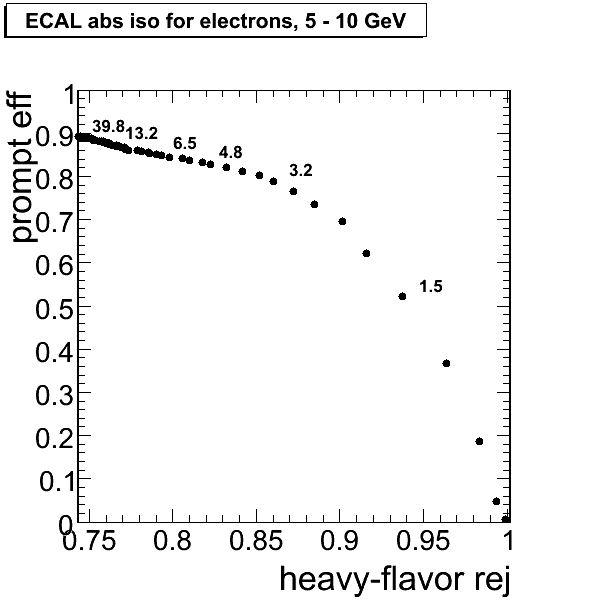
\includegraphics[width = 0.49\textwidth]{pictures/trackCut/bkgdRej_sigEff/elec_nonPrompt_ptCut0_ptCut1.png}
   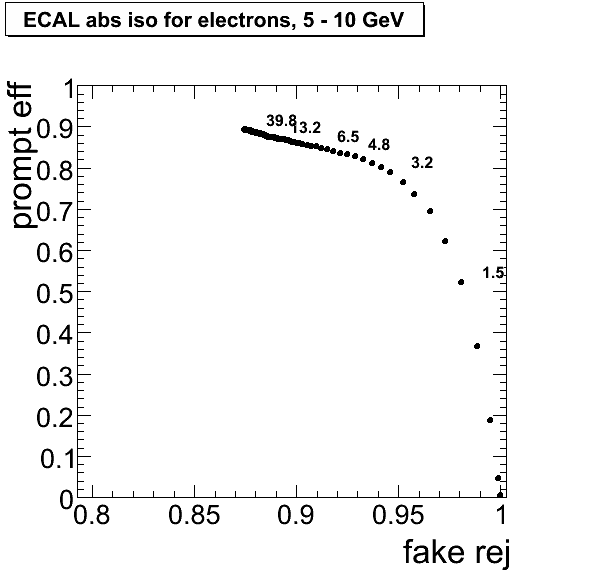
\includegraphics[width = 0.49\textwidth]{pictures/trackCut/bkgdRej_sigEff/elec_fake_ptCut0_ptCut1.png}
   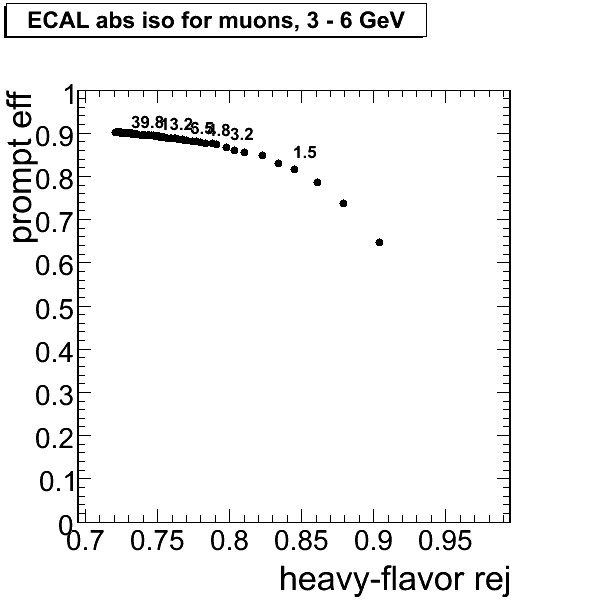
\includegraphics[width = 0.49\textwidth]{pictures/trackCut/bkgdRej_sigEff/muon_nonPrompt_ptCut0_ptCut1.png}
   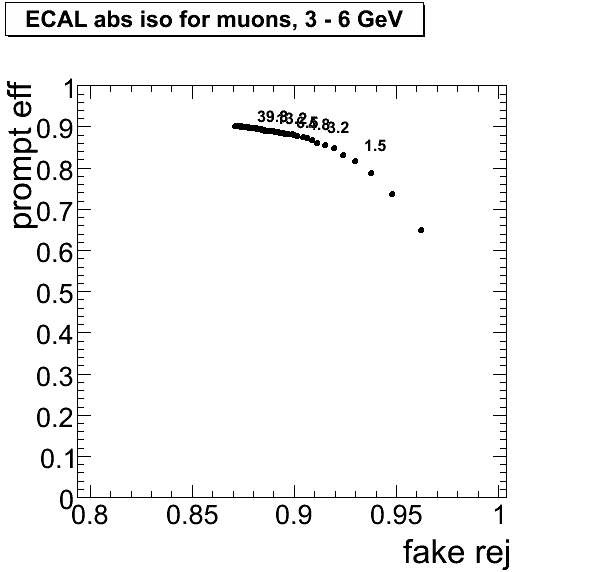
\includegraphics[width = 0.49\textwidth]{pictures/trackCut/bkgdRej_sigEff/muon_fake_ptCut0_ptCut1.png}
   \caption{\small{\label{fig:trackCut_bkgdRej_sigEff_ptCut0_ptCut1}
      Prompt lepton efficiency with respect to HF (left) and fake (right) leptons rejection
      for different cuts on ECAL isolation. Top plots are for electrons in $p_T$ range 5 -- 10 GeV after a
      tracker isolation cut of 3 GeV. Bottom plots are for  muons in $p_T$ range 3 -- 6 GeV after a tracker
      isolation cut of 5 GeV.}}
\end{center}
\end{figure}

%Figures~\ref{fig:trackCut_optEcalIsoCut_elec} and~\ref{fig:trackCut_optEcalIsoCut_muon} show
%optimized cut values as a function of the lepton transverse momentum. Here the pure$_{HF}$ and
%pure$_{fake}$ values are to be interpreted as the cuts which reject at least 90\% of the
%\textit{remaining} background leptons, after the track cut. Similarly, the efficient cut retains at
%least 90\% of the prompt leptons surviving the track cut. Thus, the overall efficiency can be
%obtained by convolving this efficiency with the efficiency of the original track cuts, shown in
%Table ???.
%
%\begin{figure}[htbp]
%\begin{center}
%   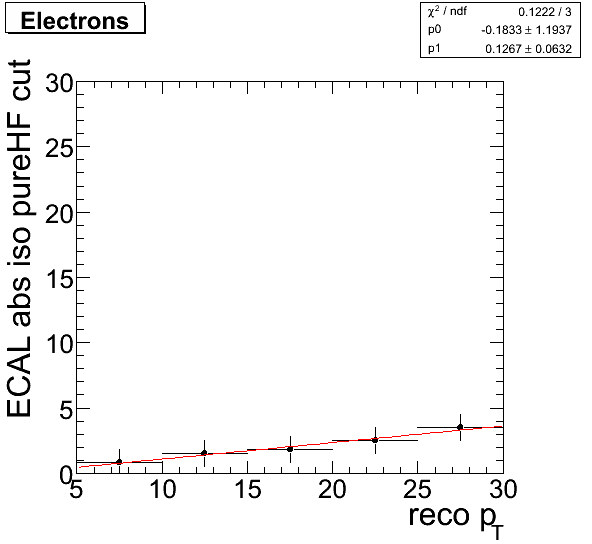
\includegraphics[width = 0.49\textwidth]{pictures/trackCut/optIsoCut/ecalIso_elec_pure_HF.png}
%   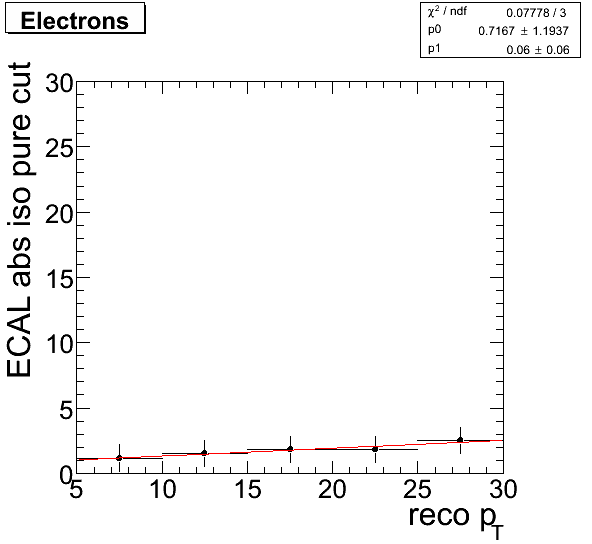
\includegraphics[width = 0.49\textwidth]{pictures/trackCut/optIsoCut/ecalIso_elec_pure.png}
%   \\
%   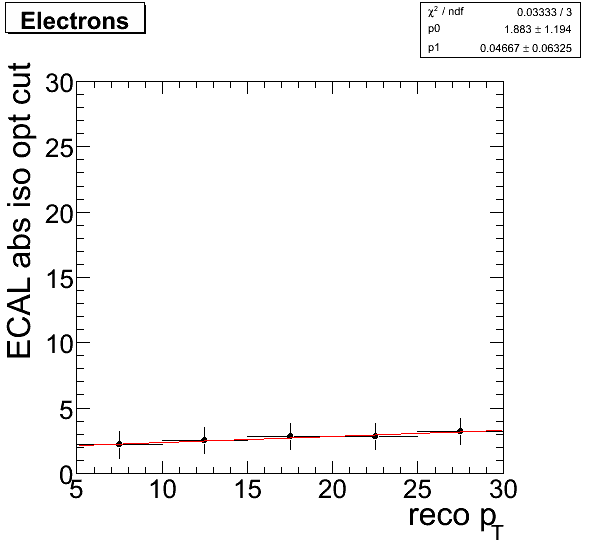
\includegraphics[width = 0.49\textwidth]{pictures/trackCut/optIsoCut/ecalIso_elec_opt.png}
%   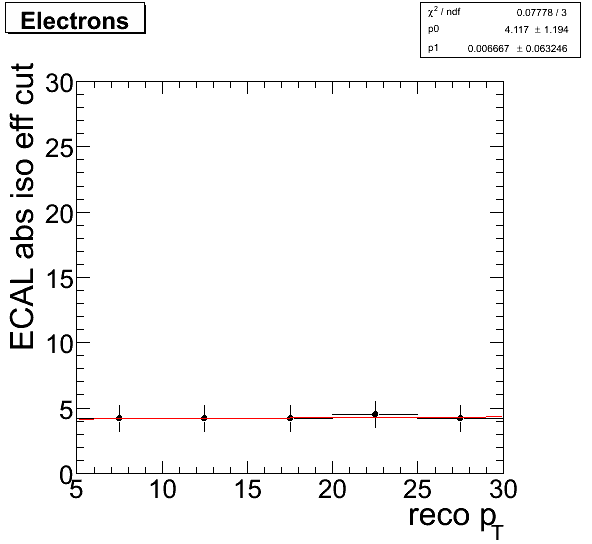
\includegraphics[width = 0.49\textwidth]{pictures/trackCut/optIsoCut/ecalIso_elec_eff.png}
%   \caption{\small{\label{fig:trackCut_optEcalIsoCut_elec}
%      ECAL isolation cut values for electrons as a function of $p_T$-bin for pure$_{HF}$ (top left),
%      pure$_{fake}$ (top right), optimal (bottom left) and efficient (bottom right) optimization
%      procedures.}}
%\end{center}
%\end{figure}

%\begin{figure}[htbp]
%\begin{center}
%   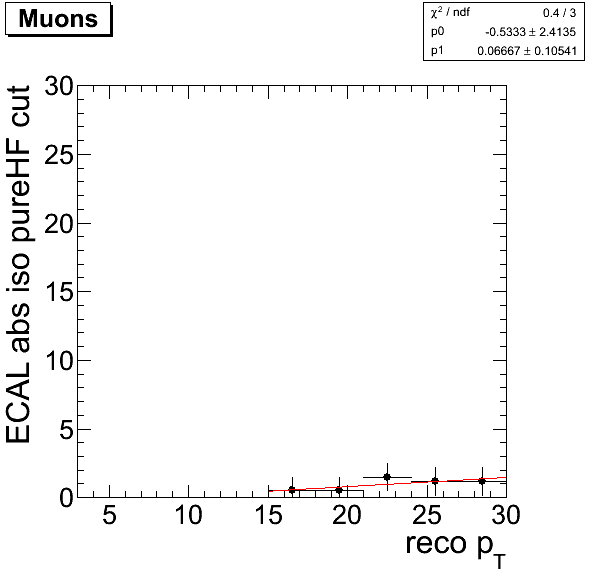
\includegraphics[width = 0.49\textwidth]{pictures/trackCut/optIsoCut/ecalIso_muon_pure_HF.png}
%   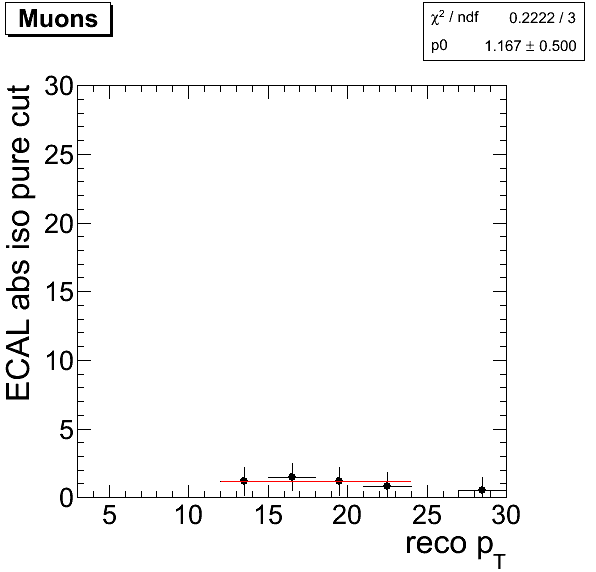
\includegraphics[width = 0.49\textwidth]{pictures/trackCut/optIsoCut/ecalIso_muon_pure.png}
%   \\
%   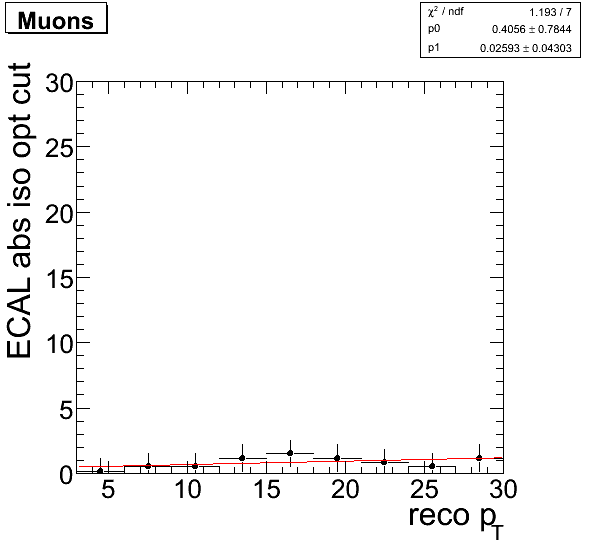
\includegraphics[width = 0.49\textwidth]{pictures/trackCut/optIsoCut/ecalIso_muon_opt.png}
%   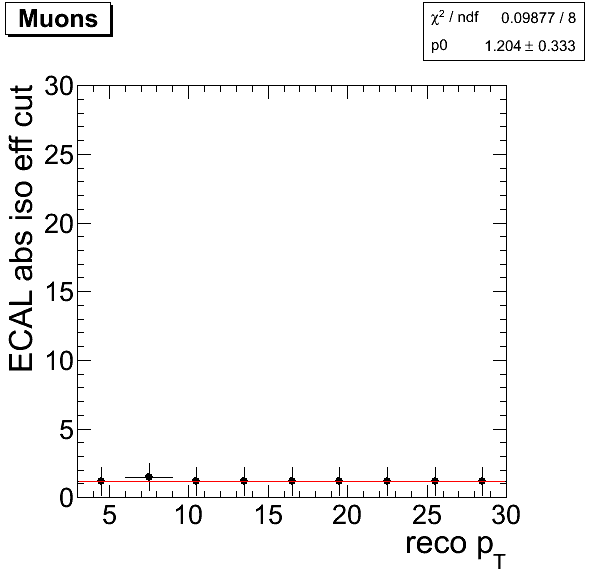
\includegraphics[width = 0.49\textwidth]{pictures/trackCut/optIsoCut/ecalIso_muon_eff.png}
%   \caption{\small{\label{fig:trackCut_optEcalIsoCut_muon}
%      ECAL isolation cut values for muons as a function of $p_T$-bin for pure$_{HF}$ (top left),
%      pure$_{fake}$ (top right), optimal (bottom left) and efficient (bottom right) optimization
%      procedures.}}
%\end{center}
%\end{figure}

%\clearpage



%\newpage

%\section{Low-$P_T$ Isolation for SUSY analysis}
%In this section the lepton isolation previously described is applied to
%two different analysis.
%The Single Lepton analysis, which could be strongly affected by a high fake lepton rate, uses the
%{\bf pure} cuts.
%The Same Sign Dilepton analysis, for which the request of two leptons reduces significantly the background
%efficiency, uses the {\bf efficient} cuts definition. In both analyses the results after the V+jets or the proposed soft
%lepton isolation ($SL$)
%are compared.
%\subsection{Single Lepton analysis}
\section{Low-$P_T$ Isolation for SUSY analysis}
%In this section the lepton isolation previously described is applied to
%two different analysis.
%For the Single Lepton analysis, which could be strongly affected by a high fake lepton rate, both the
%{\bf pure} cuts and the {\bf optimal} cuts have been applied for comparison.
%The Same Sign Dilepton analysis, for which the request of two leptons reduces significantly the background
%efficiency, uses the {\bf efficient} cuts definition. In both analyses the results after the V+jets or the proposed selection
%are compared.
The results of isolation studies described in Sec.~\ref{sec:softLepIsoOpt} were applied to
Single Lepton (SL) and Same Sign Dilepton (SSD) SUSY analyses.
For SL analysis, which is strongly affected by a high fake lepton rate, both the
{\bf pure} and the {\bf optimal} cuts have been applied for comparison. The {\bf pureFake} is applied to electrons, while the {\bf pureHF} is applied to muons, as in the muon channel the background from heavy-flavour decays is expected to be higher than that from fakes.
For SSDL analysis, for which the request of two same-sign leptons significantly increases  the background
rejection, the {\bf efficient} cuts definition was used. In both cases the results 
after applying the V+jets cuts are also shown for comparison.


\subsection{Single Lepton analysis}

The SL analysis comprise a general-purpose search for supersymmetry in events containing one-electron or one-muon in the final state, in addition to multiple jets and large missing transverse energy.

The CMS SUSY group provides a set of baseline selection criteria for the single lepton analysis in the context of the Single-lepton Reference Analysis 4 (RA4)~\cite{RA4page}. For what concerns the electron and muon isolation requirements, the RA4 suggests the standard V+jets recommendations. A comparison between the recommended V+jets isolation and the proposed Soft Lepton (SL) isolation selection is presented in terms of performance of the signal-to-background ratio and signal significance. 
 The trigger requirement of RA4 in the one-electron channel is deliberately ommitted, to allow the investigation of lowering the electron offline momentum threshold down to 5 GeV. In addition to the standard configuration of physics objects in the analysis, an official SUSY PAT Cross cleaning tool is used to correct the energy balancing for events with overlapping objects.\footnote{An electron-jet cross-cleaning is applied if an isolated electron is found close to a jet within a cone of size 0.5, whereas the muon-jet cross-cleaning is applied only if a non-isolated muon is found close to a jet (within a cone of size 0.2).}. 
 
The RA4-like cut-flow used in this analysis is the following: 

\begin{itemize}
\item $N_{lepton} = 1$
\item $N_{jets} \geq 3, \textrm{with} \;\; E_{T}^{j3} > 50 \textrm{GeV}$
\item $CaloME_{T} > 100 \textrm{GeV}$
\end{itemize}

The Monte Carlo (MC) data samples with the corresponding statistics, are listed in Table~\ref{tab:SLsamples}. The SM background processes are produced with the Madgraph MC generator, and include W+jets, $t \bar{t}$, as well as QCD N-jet events.

\begin{table}[htb]

\begin{center}
\begin{tabular}{|c|c|c|}
\hline
Sample  &  N MC events & $\sigma$ (pb) \\
\hline
SUSY (LM0) & 202686 & 110\\
SUSY (LM1) & 104800 & 16.06\\
\hline
QCD, 250 $<\hat{pT}<$ 500 GeV  & 4874539 & 400000\\
QCD, 500 $<\hat{pT}<$ 1000 GeV  & 4570718 & 14000\\
QCD, $\hat{pT}>$ 1000 GeV  & 1046863 & 370 \\ \hline
$b\bar{b}$+jets, 250 $<\hat{pT}<$ 500 GeV  & 1052158 & 15000\\
$b\bar{b}$+jets, 500 $<\hat{pT}<$ 1000 GeV  & 985233 & 700\\
$b\bar{b}$+jets, $\hat{pT}>$ 1000 GeV  & 327618 & 13  \\
\hline
W+ jets&8900000 & 40000 \\
\hline
$t \bar{t}$+jets& 946644& 317 \\
\hline
\end{tabular}
\caption{\small{MC samples used in the SL analysis.}\label{tab:SLsamples}}
\end{center}
\end{table}


In table~\ref{tab:SLres} the number of signal and background events is compared between the {\bf optimal} SL isolation selection and the one recommended by the
V + jets group for leptons with $P_{T} > 10$ GeV. Further results are also provided for leptons with $P_{T}>5$GeV. In the final two rows the significance is reported for LM0 and LM1 respectively. The corresponding numbers when applying the {\bf pureHF} cuts to muons and {\bf pureFake} cu8ts to electrons are shown in table~\ref{tab:SLres2}.

For both the electron and muon channels, the proposed {\bf pure} and {\bf optimal} SL isolation cuts produce a significant increase in the signal yield, since these cuts appear rather loose compared to the V+jets ones. The number of background events is increased as well, particularly from QCD processes. The {\bf optimal} cuts show higher significance values than the {\bf pure} for both muons and electrons.

In the electron channel, the significance increases while applying the SL isolation, despite the steep increase of QCD. The muon channel shows similarly an increase in the signal significance, mainly pronounced in the LM0 case. The move to a 5GeV lepton $P_{T}$ threshold shows some improvement for muons, although this is minimal due to the reduced efficiency in the muon reconstruction (for muons below 10 GeV). In the electrons case, the significance reduces for LM0, and is barely improved for LM1. This indicates that switching to a threshold of 5GeV in the electron momentum may not be beneficial.

The above event yield comparison confirms that it is possible to improve the signal significance of the single lepton analysis whilst using low-$P_{T}$ leptons. The soft lepton isolation performance shows comparable significance between the {\bf optimal} and the {\bf pure} selection. In the 1-muon channel, the attempt of lowering the muon momentum threshold to 5GeV $P_{T}$ shows a profitable gain in the signal significance, whereas in the 1-electron, the maintenance of the 10 GeV threshold may be preferable.


\begin{table}[htb]
\begin{center}
\begin{tabular}{|c||c|c|c||c|c|c|}
\hline
Sample  & \multicolumn{3}{|c||} {$e$} & \multicolumn{3}{|c|} {$\mu$} \\
\hline
 & V+j$_{pt_{10}}$ & SL$_{{\bf opt}:pt_{10}}$  & SL$_{{\bf opt}:pt_{5}}$ & V+j$_{pt_{10}}$ & SL$_{{\bf opt}:pt_{10}}$  & SL$_{{\bf opt}:pt_{5}}$ \\
\hline
SUSY(LM0) & 364.0 & 423.1 & 426.1 & 512.5 & 604.0 & 709.8 \\
\hline
SUSY(LM1) & 58.5 & 73.9  & 78.4 & 87.0 & 97.7 & 124.2\\
\hline
$t\bar{t}$ & 278.6 & 328.8 & 334.2 & 376.7 & 424.0  & 467.7 \\
\hline
W+jets & 159.7 & 192.1 & 198.7 & 182.2 & 206.5 & 229.0\\
\hline
QCD (250-500) & 0.0 & 8.2 & 8.2 & 0.0 & 41.0 & 73.9 \\
\hline
QCD (500-1000) & 1.2 & 2.5 & 5.5 & 1.2 & 34.6 & 84.8 \\
\hline
QCD (1000-inf) & 0.5 & 0.9 & 1.3 & 0.1 & 2.5 & 8.8 \\
\hline
$b\bar{b}+\textrm{jets}$ (250-500) & 0.0 & 0.0 & 0.0 & 1.4 & 15.7 & 37.1 \\
\hline 
$b\bar{b}+\textrm{jets}$ (500-1000) & 0.1 & 0.8 & 0.5 & 0.4 & 12.4 & 28.1 \\
\hline
$b\bar{b}+\textrm{jets}$ (1000-inf) & 0.1 & 0.1 & 0.1 & 0.1 & 0.8 & 1.7 \\ 
\hline
\hline
$S/\sqrt{S+B}$ (LM0) & 17.3  & 18.3 & 18.2 & 21.6 & 22.2 & 23.2\\
\hline
$S/\sqrt{S+B}$ (LM1) & 2.8 & 3.2 & 3.4 & 3.7 & 3.6& 4.1 \\
\hline

\end{tabular}
\caption{\small{Number of events in the single electron and muon final states, for $100\textrm{pb}^{-1}$ of integrated luminosity,
	for the V + jets and the proposed {\bf optimal} soft lepton isolation (SL).
The lepton $p_T$ cut for the V + jets and SL$_{{\bf opt}:pt_{10}}$
is 10 GeV while $SL_{{\bf opt}:pt_{5}}$  is 5 Gev.
 In the last two rows the significance is reported for both LM0 and LM1}\label{tab:SLres}}
\end{center}
\end{table}



\begin{table}[htb]
\begin{center}
\begin{tabular}{|c||c|c|c||c|c|c|}
\hline
Sample  & \multicolumn{3}{|c||} {$e$} & \multicolumn{3}{|c|} {$\mu$} \\
\hline
 & V+j$_{pt_{10}}$ & SL$_{{\bf pur}:pt_{10}}$  & SL$_{{\bf pur}:pt_{5}}$ & V+j$_{pt_{10}}$ & SL$_{{\bf pur}:pt_{10}}$  & SL$_{{\bf pur}:pt_{5}}$ \\
 \hline
SUSY(LM0) & 364.0 & 417.8 & 418.2 & 512.5 & 584.2  & 665.09 \\
\hline
SUSY(LM1) & 58.5 & 73.5  & 77.6 & 87.0  & 95.8 & 120.4 \\
\hline
$t\bar{t}$ & 278.6 &325.0 &327.8 & 376.7 & 418.2 & 456.5 \\
\hline
W+jets & 159.7 &192.1  & 198.7 & 182.2 & 205.6 & 226.6 \\
\hline
QCD (250-500) & 0.0 & 8.2 & 8.2 & 0.0 & 24.6 & 41.0 \\
\hline
QCD (500-1000) & 1.2 & 2.5 & 5.2 & 1.2 & 23.6 & 50.5 \\
\hline
QCD (1000-inf) & 0.5 & 0.9 & 1.3 & 0.1 & 1.8  & 5.8 \\
\hline
$b\bar{b}+\textrm{jets}$ (250-500) & 0.0 & 0.0 & 0.0 & 1.4 & 11.4 & 25.7 \\
\hline 
$b\bar{b}+\textrm{jets}$ (500-1000) & 0.1 & 0.5 & 0.8 & 0.4 & 8.6 & 18.7 \\
\hline
$b\bar{b}+\textrm{jets}$ (1000-inf) & 0.1 & 0.1 & 0.1 & 0.1 & 0.6 & 1.2 \\ 
\hline
\hline
$S/\sqrt{S+B}$ (LM0) & 17.3 & 18.2 & 18. & 21.6 & 22.2 & 23.1\\
\hline
$S/\sqrt{S+B}$ (LM1) & 2.8 & 3.2 & 3.3 & 3.7 & 3.6 & 4.2 \\
\hline

\end{tabular}
\caption{\small{Number of events in the single electron and muon final states, for $100\textrm{pb}^{-1}$ of integrated luminosity, 
	for the V + jets and the proposed {\bf pure} soft lepton isolation (SL) ({\bf pureHF} for muons, and {\bf pureFake} for electrons).
The lepton $p_T$ cut for the V + jets and SL$_{{\bf pur}:pt_{10}}$
is 10 GeV while $SL_{{\bf pur}:pt_{5}}$  is 5 Gev.
 In the last two rows the significance is reported for both LM0 and LM1}\label{tab:SLres2}}
\end{center}
\end{table}

\subsection{Same Sign DiLepton analysis}
The SSDL analysis comprise a general-purpose search for supersymmetry in events containing two same sign
leptons of any combination of flavors,
in addition to multiple jets and large missing transverse energy. The requirement of two same sign
leptons significantly reduces the background contribution and provides very clear signature for discovery of SUSY
at LHC.

The CMS SUSY group provides a set of baseline selection criteria for Single-lepton Reference Analysis 5 (RA5)~\cite{RA5page}.  A complete description of the SSDL analysis strategy and
selection can be found elsewhere~\cite{ssdlnote}.
In addition to the standard configuration of physics objects in the analysis, we introduce the usage of the official SUSY PAT Cross cleaning tool.


To select events the following basic cuts were applied:
\begin{itemize}
\item MET trigger (MET $>$ 50 GeV)
\item $HT= >$ 350 GeV
\item $N_{lept} >$ 1
\item First and second lepton (classified in $p_T$) with same charge
\end{itemize}

The samples used for this study are reported in Tab.~\ref{tab:SSDLsamples}.
\begin{table}[htb]

\begin{center}
\begin{tabular}{|c|c|c|}
\hline
Sample  &  N MC events & $\sigma$ (pb) \\
\hline
SUSY (LM0) & 202686 & 110\\
SUSY (LM1) & 104800 & 15.06\\
\hline
QCD 80 $<\hat{pt}<$ 170 GeV&3437680 & 1934640\\
QCD 170 $<\hat{pt}<$ 300 GeV &3746780 & 62563\\
QCD 300 $<\hat{pt}<$ 470 GeV & 1810585& 3665\\
QCD 470 $<\hat{pt}<$ 800 GeV &2406752 & 316\\
QCD 800 $<\hat{pt}<$ 1400 GeV &2907476	 & 11.9\\
QCD 1400 $<\hat{pt}<$ 2200 GeV &584256 & 0.172\\
QCD 2200 $<\hat{pt}<$ 3000 GeV &878796 & 0.00142\\
QCD $\hat{pt}>$ 3000 GeV &567040 & 0.0000086\\
\hline
W+ jets&8900000 & 40000 \\
\hline
Z+jets& 1262816& 3700\\
\hline
$t \bar{t}$+jets& 946644& 317 \\
\hline
WW  & 204722 & 44.8 \\
ZZ & 199810 & 17.4 \\
WZ &246550 & 7.1\\
WW (same sign DPS) &1000 & 0.0216\\
\hline
\end{tabular}
\caption{\small{MonteCarlo samples analyzed for the search of the SSDL events.}\label{tab:SSDLsamples}}
\end{center}
\end{table}


In table~\ref{tab:SSDLres} the number of signal and background events
expected at 10 TeV with 100 pb$^{-1}$
with the proposed lepton selection
is compared with the results of the recommended selection by the
V + jets group (with $P_t >$ 10 GeV).
Final states with taus will not be considered for this comparison.

\begin{table}[htb]
\begin{center}
\begin{tabular}{|c||c|c|c||c|c|c||c|c|c|}
\hline
Sample &\multicolumn{3}{|c||} {$e e$} &\multicolumn{3}{|c||} {$\mu \mu$} &\multicolumn{3}{|c|} {$ e \mu$} \\
\hline
 & V+j$_{pt_{10}}$ & SL$_{pt_{10}}$  & SL$_{pt_{5}}$ & V+j$_{pt_{10}}$ & SL$_{pt_{10}}$  & SL$_{pt_{5}}$ & V+j$_{pt_{10}}$ & SL$_{pt_{10}}$  & SL$_{pt_{5}}$  \\
\hline
SUSY(LM0) &2.44 &4.23 &4.67 &9.99 &16.28 &28.87 &10.47 &16.99 & 22.95\\
\hline
SUSY(LM1) &0.52 &1.10 &1.30 &2.15 &3.03&5.46 &2.84 &3.94 &5.61 \\
\hline
$t\bar{t}$ &0.07 &0.20 & 0.33 &0.13 &1.88 &7.20 &0.23 &1.58 & 3.75\\
\hline
W/Z + jets &0.00 &0.00 &0.00 &0.00 &0.00 &0.00 &0.00 & 0.00 & 0.45\\
\hline
diBosons &0.02 &0.02 &0.02 &0.02 &0.13 &0.03 &0.01 & 0.01 & 0.04\\
\hline
QCD &0.00 &0.00 &0.00 &0.00 &0.20 &5.64 &0.00 & 0.00 & 1.93\\
\hline \hline
$S/\sqrt{S+B}$ (LM0)  &1.5 &2.0  &2.1 &3.1 &3.8 &4.4  &3.2 &3.9  & 4.3\\
\hline \hline
$S/\sqrt{S+B}$ (LM1)  &0.7 &1.0 &1.0 &1.4 &1.3 &1.3  &1.6 &1.7  &1.6\\
\hline
\end{tabular}
\caption{\small{Number of events in the final states $e e$, $\mu \mu$, $ e \mu$,
	for the V + jets and the proposed soft lepton isolation (SL).
The lepton $p_T$ cut for the V + jets and SL$_{pt_{10}}$
is 10 GeV while SL$_{pt_{5}}$  is 5 Gev.
 In the last row the significance is reported.}\label{tab:SSDLres}}
\end{center}
\end{table}
%As can be seen from Table~\ref{tab:SSDLres} moving from V+j$_{pt_{10}}$  to SL$_{pt_{10}}$ increases 
%significantly the signal yield....



%\newpage



\section{Summary}
\label{sec:Summary}

This study proposes two methods of data-driven QCD background estimation, and presents results from Monte Carlo and the first X pb$^{-1}$ of 7TeV data taken by CMS at the LHC. 

Following the promising results of studies into using the $\alpha_{T}$  kinematic variable in the single electron mode of SUSY searches, it is proposed that a suitable control sample in the distribution of this variable for predicting the QCD background could be obtained by inverting the $\Delta \phi$ and $\Delta \eta$ cuts in the electron selection criteria. 

The analysis uses Monte Carlo samples to perform a closure test on this method, first with a pure QCD sample, and then with W + jets contamination in the anti-selected control sample. The method proved unbiased between selected and anti-selected in these tests. 

The first look at this method under 7TeV collision data and corresponding Monte Carlo is also shown, with lowered selection to maximise available statistics.



\appendix

%\clearpage

%\section{Tracker Isolation Plots for all the $p_T$ bins}


In this note we will consider separate optimization of each isolation component individually, and
examine the effect of consecutive cuts.

Absolute isolation is shown in
Fig.~\ref{fig:PromptElecRecoPt_AbsIso} separately for each isolation variable as a function
of reconstructed $p_T$ for electrons and in Fig.... for muons. The`relative
isolation is shown in Fig.~\ref{fig:PromptElecRecoPt_RelIso} and Fig...., for electrons and
muons respectively.

 Particularly for soft electrons, the
 `explicit dependence of relative isolation on $p_T$ becomes apparent, while absolute isolation
 remains relatively constant across $p_T$ bins. Thus, for soft electrons we seek to optimize absolute
 isolation.

 \begin{figure}[htbp]
    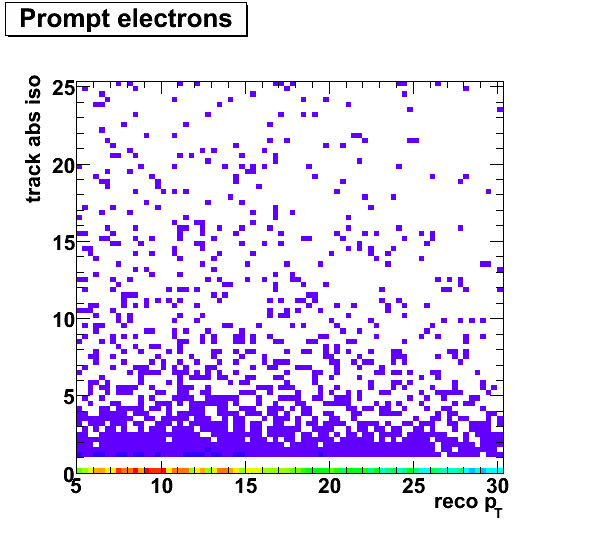
\includegraphics[width = 0.33\textwidth]{pictures/recoPt_absIso/trackIso_elec_prompt.png}
    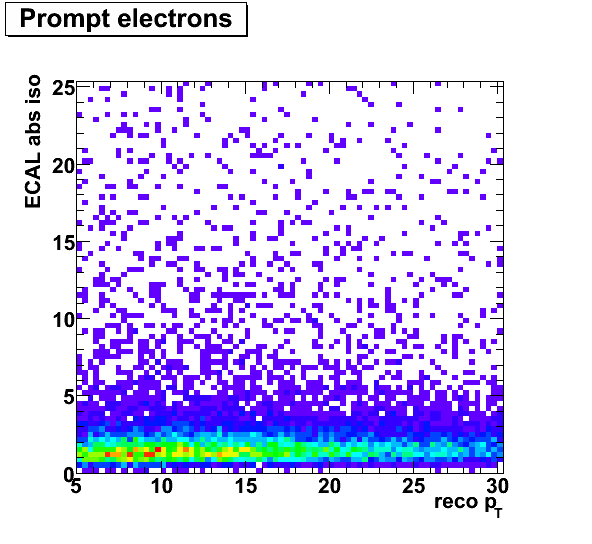
\includegraphics[width = 0.33\textwidth]{pictures/recoPt_absIso/ecalIso_elec_prompt.png}
    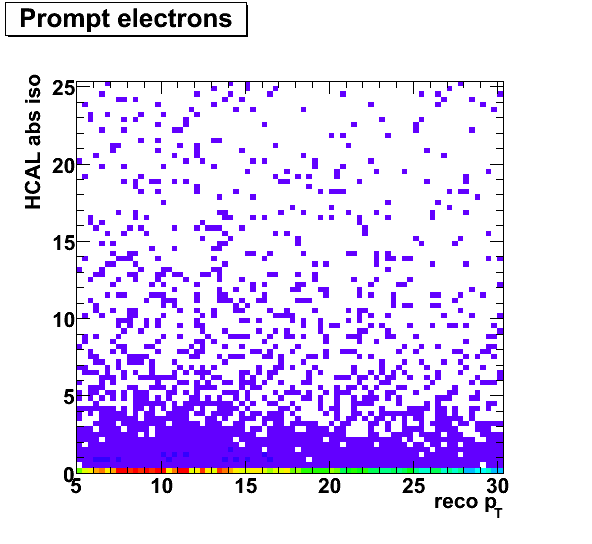
\includegraphics[width = 0.33\textwidth]{pictures/recoPt_absIso/hcalIso_elec_prompt.png}
    \caption{Absolute isolation calculated from (a) tracker, (b) ECAL and (c) HCAL as a function
       of reconstructed $p_{T}$ for prompt electrons}
    \label{fig:PromptElecRecoPt_AbsIso}
 \end{figure}

 \begin{figure}[htbp]
    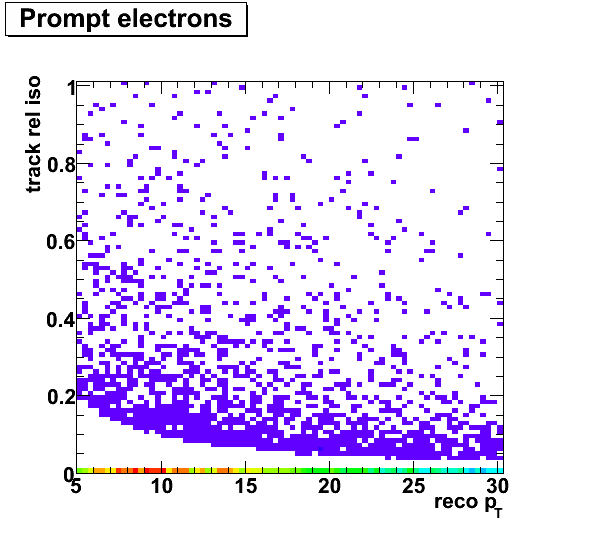
\includegraphics[width = 0.33\textwidth]{pictures/recoPt_relIso/trackIso_elec_prompt.png}
    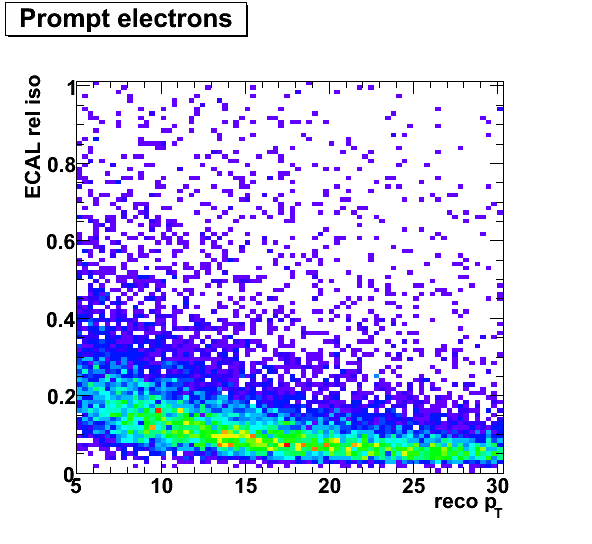
\includegraphics[width = 0.33\textwidth]{pictures/recoPt_relIso/ecalIso_elec_prompt.png}
    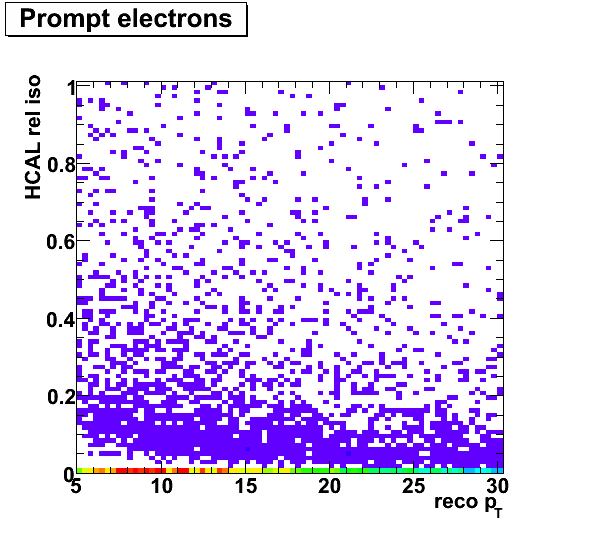
\includegraphics[width = 0.33\textwidth]{pictures/recoPt_relIso/hcalIso_elec_prompt.png}
    \caption{Relative isolation calculated from (a) tracker, (b) ECAL and (c) HCAL as a function of
       reconstructed $p_{T}$ for prompt electrons}
    \label{fig:PromptElecRecoPt_RelIso}
 \end{figure}

 \clearpage

 \begin{figure}[htbp]
    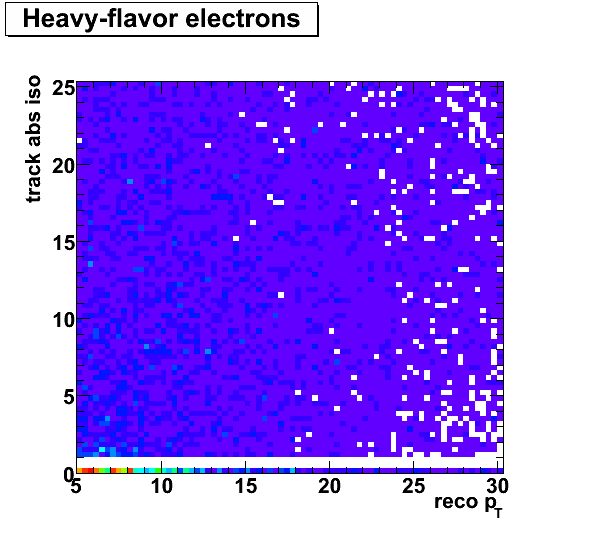
\includegraphics[width = 0.33\textwidth]{pictures/recoPt_absIso/trackIso_elec_nonPrompt.png}
    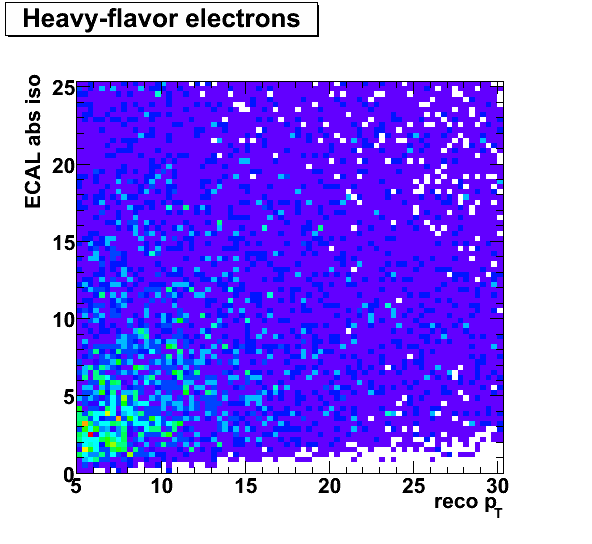
\includegraphics[width = 0.33\textwidth]{pictures/recoPt_absIso/ecalIso_elec_nonPrompt.png}
    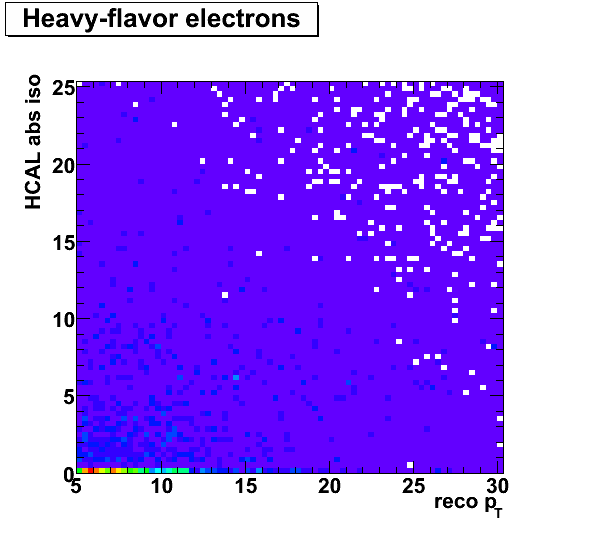
\includegraphics[width = 0.33\textwidth]{pictures/recoPt_absIso/hcalIso_elec_nonPrompt.png}
    \caption{Absolute isolation calculated from (a) tracker, (b) ECAL and (c) HCAL as a function of
       reconstructed $p_{T}$ for non-prompt electrons}
    \label{fig:NonPromptElecRecoPt_AbsIso}
 \end{figure}

 \begin{figure}[htbp]
    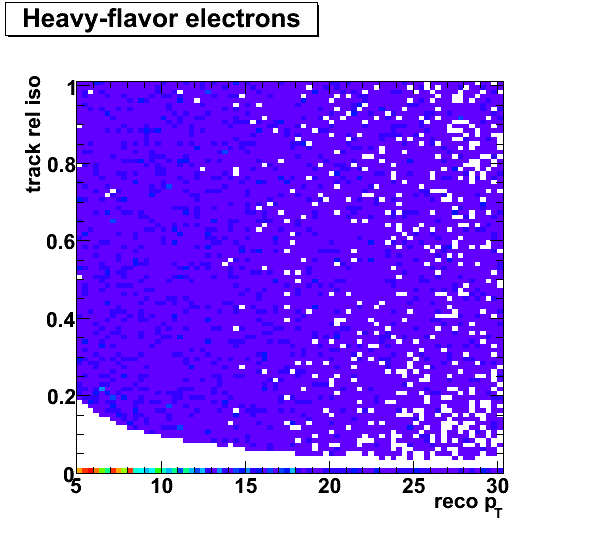
\includegraphics[width = 0.33\textwidth]{pictures/recoPt_relIso/trackIso_elec_nonPrompt.png}
    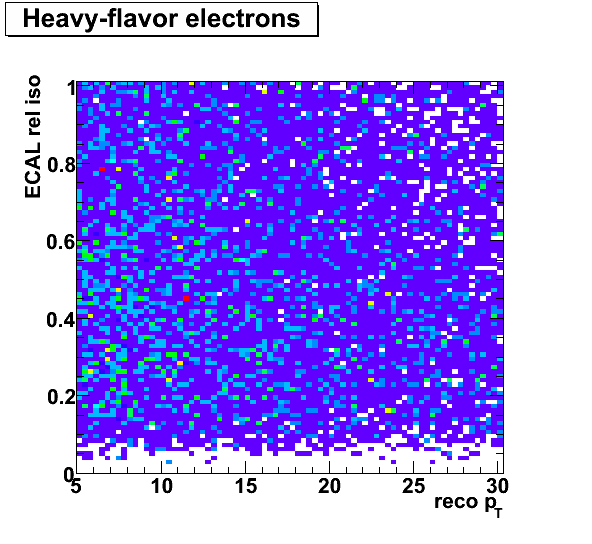
\includegraphics[width = 0.33\textwidth]{pictures/recoPt_relIso/ecalIso_elec_nonPrompt.png}
    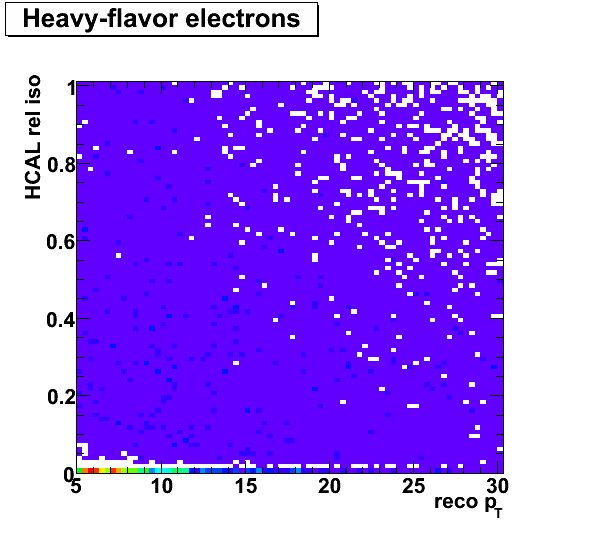
\includegraphics[width = 0.33\textwidth]{pictures/recoPt_relIso/hcalIso_elec_nonPrompt.png}
    \caption{Relative isolation calculated from (a) tracker, (b) ECAL and (c) HCAL as a function of
       reconstructed $p_{T}$ for non-prompt electrons}
    \label{fig:NonPromptElecRecoPt_RelIso}
 \end{figure}

 \clearpage

 \begin{figure}[htbp]
    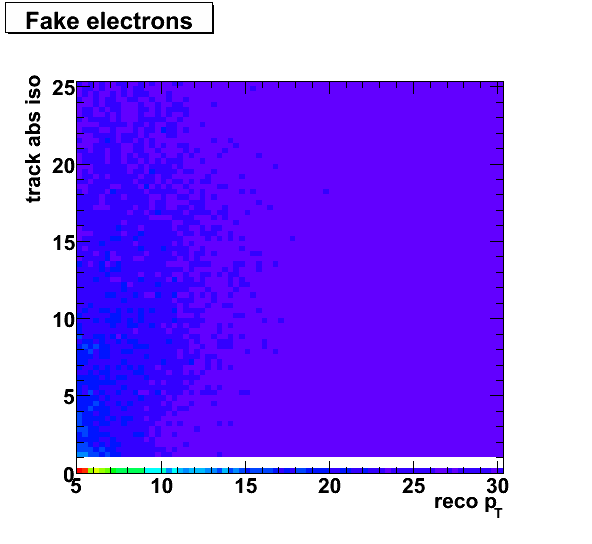
\includegraphics[width = 0.33\textwidth]{pictures/recoPt_absIso/trackIso_elec_fake.png}
    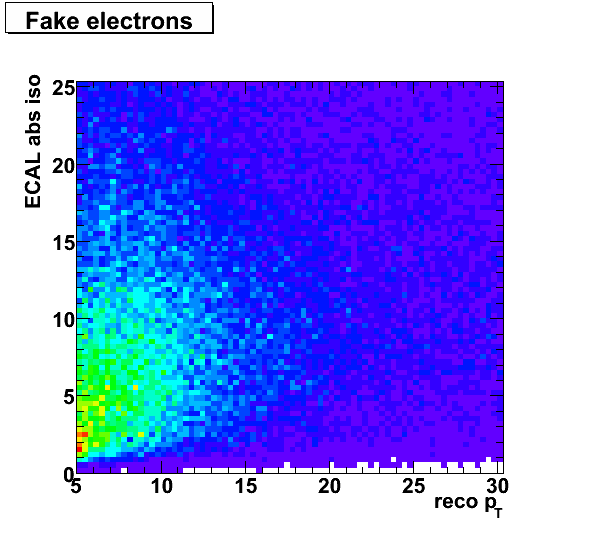
\includegraphics[width = 0.33\textwidth]{pictures/recoPt_absIso/ecalIso_elec_fake.png}
    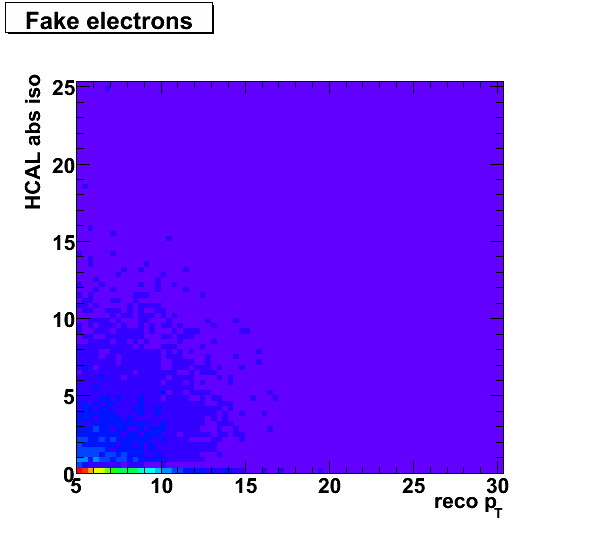
\includegraphics[width = 0.33\textwidth]{pictures/recoPt_absIso/hcalIso_elec_fake.png}
    \caption{Absolute isolation calculated from (a) tracker, (b) ECAL and (c) HCAL  as a function of
       reconstructed $p_{T}$ for fake electrons}
    \label{fig:FakeElecRecoPt_AbsIso}
 \end{figure}

 \begin{figure}[htbp]
    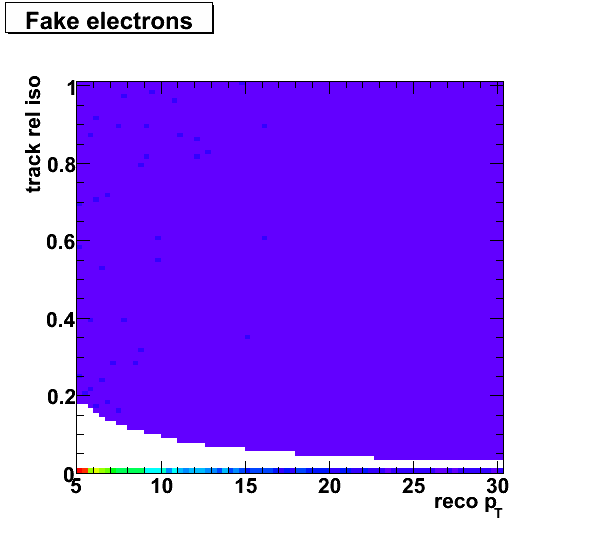
\includegraphics[width = 0.33\textwidth]{pictures/recoPt_relIso/trackIso_elec_fake.png}
    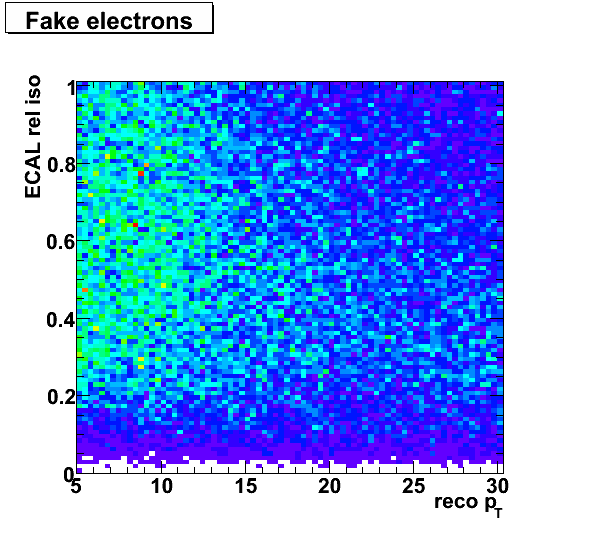
\includegraphics[width = 0.33\textwidth]{pictures/recoPt_relIso/ecalIso_elec_fake.png}
    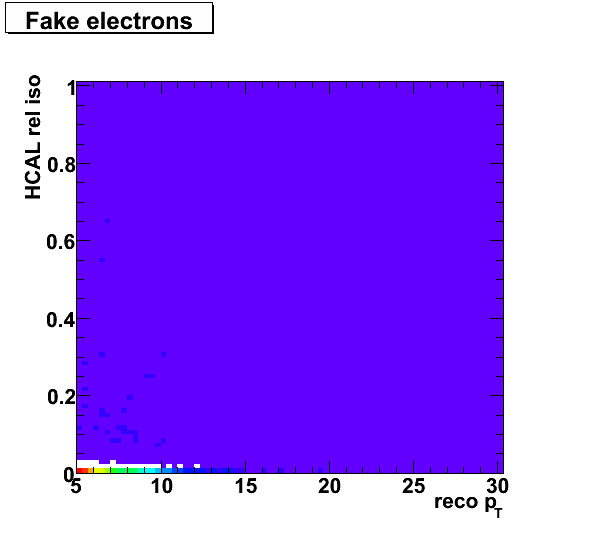
\includegraphics[width = 0.33\textwidth]{pictures/recoPt_relIso/hcalIso_elec_fake.png}
    \caption{Relative isolation calculated from (a) tracker, (b) ECAL and (c) HCAL as a function of
       reconstructed $p_{T}$ for fake electrons}
    \label{fig:FakeElecRecoPt_RelIso}
 \end{figure}

 \clearpage

 \begin{figure}[htbp]
    \includegraphics[width = 0.33\textwidth]{pictures/recoPt_absIso/trackIso_muon_prompt.png}
    \includegraphics[width = 0.33\textwidth]{pictures/recoPt_absIso/ecalIso_muon_prompt.png}
    \includegraphics[width = 0.33\textwidth]{pictures/recoPt_absIso/hcalIso_muon_prompt.png}
    \caption{Absolute isolation calculated from (a) tracker, (b) ECAL and (c) HCAL versus
       reconstructed $p_{T}$ for prompt muons}
    \label{fig:PromptMuonRecoPt_AbsIso}
 \end{figure}

 \begin{figure}[htbp]
    \includegraphics[width = 0.33\textwidth]{pictures/recoPt_relIso/trackIso_muon_prompt.png}
    \includegraphics[width = 0.33\textwidth]{pictures/recoPt_relIso/ecalIso_muon_prompt.png}
    \includegraphics[width = 0.33\textwidth]{pictures/recoPt_relIso/hcalIso_muon_prompt.png}
    \caption{Relative isolation calculated from (a) tracker, (b) ECAL and (c) HCAL versus
       reconstructed $p_{T}$ for prompt muons}
    \label{fig:PromptMuonRecoPt_RelIso}
 \end{figure}

 \clearpage

 \begin{figure}[htbp]
    \includegraphics[width = 0.33\textwidth]{pictures/recoPt_absIso/trackIso_muon_nonPrompt.png}
    \includegraphics[width = 0.33\textwidth]{pictures/recoPt_absIso/ecalIso_muon_nonPrompt.png}
    \includegraphics[width = 0.33\textwidth]{pictures/recoPt_absIso/hcalIso_muon_nonPrompt.png}
    \caption{Absolute isolation calculated from (a) tracker, (b) ECAL and (c) HCAL versus
       reconstructed $p_{T}$ for hadronic muons}
    \label{fig:NonPromptMuonRecoPt_AbsIso}
 \end{figure}

 \begin{figure}[htbp]
    \includegraphics[width = 0.33\textwidth]{pictures/recoPt_relIso/trackIso_muon_nonPrompt.png}
    \includegraphics[width = 0.33\textwidth]{pictures/recoPt_relIso/ecalIso_muon_nonPrompt.png}
    \includegraphics[width = 0.33\textwidth]{pictures/recoPt_relIso/hcalIso_muon_nonPrompt.png}
    \caption{Relative isolation calculated from (a) tracker, (b) ECAL and (c) HCAL versus
       reconstructed $p_{T}$ for hadronic muons}
    \label{fig:NonPromptMuonRecoPt_RelIso}
 \end{figure}

 \clearpage

 \begin{figure}[htbp]
    \includegraphics[width = 0.33\textwidth]{pictures/recoPt_absIso/trackIso_muon_fake.png}
   \includegraphics[width = 0.33\textwidth]{pictures/recoPt_absIso/ecalIso_muon_fake.png}
    \includegraphics[width = 0.33\textwidth]{pictures/recoPt_absIso/hcalIso_muon_fake.png}
    \caption{Absolute isolation calculated from (a) tracker, (b) ECAL and (c) HCAL versus
       reconstructed $p_{T}$ for fake muons}
    \label{fig:FakeMuonRecoPt_AbsIso}
 \end{figure}

 \begin{figure}[htbp]
    \includegraphics[width = 0.33\textwidth]{pictures/recoPt_relIso/trackIso_muon_fake.png}
    \includegraphics[width = 0.33\textwidth]{pictures/recoPt_relIso/ecalIso_muon_fake.png}
    \includegraphics[width = 0.33\textwidth]{pictures/recoPt_relIso/hcalIso_muon_fake.png}
    \caption{Relative isolation calculated from (a) tracker, (b) ECAL and (c) HCAL versus
       reconstructed $p_{T}$ for fake muons}
    \label{fig:FakeMuonRecoPt_RelIso}
 \end{figure}

 \clearpage

 Figure~\ref{fig:AbsIsoCut_CutEffRej_Elec_PtCut0_PtCut1} shows the signal efficiency / background
 rejection of a cut on absolute isolation for electrons between 5 and 10 GeV.
 Figure~\ref{fig:AbsIsoCut_CutEffRej_Elec_PtCut4_PtCut5} shows these same curves for electrons
 between 25 and 30 GeV. We examine each $p_T$ range independently in order to optimize our isolation
 cut bin-by-bin.

 \begin{figure}[htbp]
    \includegraphics[width = 0.33\textwidth]{pictures/absIsoCut_absIsoCutEff/absIsoCut_trackIso_cutEff_elec_ptCut0_ptCut1.png}
    \includegraphics[width = 0.33\textwidth]{pictures/absIsoCut_absIsoCutEff/absIsoCut_ecalIso_cutEff_elec_ptCut0_ptCut1.png}
    \includegraphics[width = 0.33\textwidth]{pictures/absIsoCut_absIsoCutEff/absIsoCut_hcalIso_cutEff_elec_ptCut0_ptCut1.png}
    \caption{Signal efficiency and background rejection ($1 -$ eff) of a cut on absolute isolation
       calculated from (a) the tracker, (b) the ECAL and (c) the HCAL for electrons with a
       reconstructed $p_{T}$ from 5 -- 10 GeV. The first curve indicates the efficiency for prompt
       electrons, the second curve indicates the rejection for hadronic electrons, and the third
       curve indicates the rejection for fake electrons.}
    \label{fig:AbsIsoCut_CutEffRej_Elec_PtCut0_PtCut1}
 \end{figure}

 \begin{figure}[htbp]
    \includegraphics[width = 0.33\textwidth]{pictures/absIsoCut_absIsoCutEff/absIsoCut_trackIso_cutEff_elec_ptCut4_ptCut5.png}
    \includegraphics[width = 0.33\textwidth]{pictures/absIsoCut_absIsoCutEff/absIsoCut_ecalIso_cutEff_elec_ptCut4_ptCut5.png}
    \includegraphics[width = 0.33\textwidth]{pictures/absIsoCut_absIsoCutEff/absIsoCut_hcalIso_cutEff_elec_ptCut4_ptCut5.png}
    \caption{Signal efficiency and background rejection ($1 -$ eff) of a cut on absolute isolation
       calculated from (a) the tracker, (b) the ECAL and (c) the HCAL for electrons with a
       reconstructed $p_{T}$ from 25 -- 30 GeV. The first curve indicates the efficiency for prompt
       electrons, the second curve indicates the rejection for hadronic electrons, and the third
       curve indicates the rejection for fake electrons.}
    \label{fig:AbsIsoCut_CutEffRej_Elec_PtCut4_PtCut5}
 \end{figure}

 \clearpage

 \begin{figure}[htbp]
    \includegraphics[width = 0.33\textwidth]{pictures/absIsoCut_absIsoCutEff/absIsoCut_trackIso_cutEff_muon_ptCut0_ptCut1.png}
    \includegraphics[width = 0.33\textwidth]{pictures/absIsoCut_absIsoCutEff/absIsoCut_ecalIso_cutEff_muon_ptCut0_ptCut1.png}
    \includegraphics[width = 0.33\textwidth]{pictures/absIsoCut_absIsoCutEff/absIsoCut_hcalIso_cutEff_muon_ptCut0_ptCut1.png}
    \caption{Signal efficiency and background rejection ($1 - $ eff) of a cut on absolute isolation
       calculated from (a) the tracker, (b) the ECAL and (c) the HCAL for muons with a reconstructed
       $p_{T}$ from 3 -- 6 GeV. The first curve indicates the efficiency for prompt muons, the second
       curve indicates the rejection for hadronic muons, and the third curve indicates the rejection
       for fake muons.}
    \label{fig:AbsIsoCut_CutEffRej_Muon_PtCut0_PtCut1}
 \end{figure}

\begin{figure}[htbp]
   \includegraphics[width = 0.33\textwidth]{pictures/absIsoCut_absIsoCutEff/absIsoCut_trackIso_cutEff_muon_ptCut8_ptCut9.png}
   \includegraphics[width = 0.33\textwidth]{pictures/absIsoCut_absIsoCutEff/absIsoCut_ecalIso_cutEff_muon_ptCut8_ptCut9.png}
   \includegraphics[width = 0.33\textwidth]{pictures/absIsoCut_absIsoCutEff/absIsoCut_hcalIso_cutEff_muon_ptCut8_ptCut9.png}
   \caption{Signal efficiency and background rejection ($1 - $ eff) of a cut on absolute isolation
      calculated from (a) the tracker, (b) the ECAL and (c) the HCAL for muons with a reconstructed
      $p_{T}$ from 15 -- 18 GeV. The first curve indicates the efficiency for prompt muons, the
      second curve indicates the rejection for hadronic muons, and the third curve indicates the
      rejection for fake muons.}
   \label{fig:AbsIsoCut_CutEffRej_Muon_PtCut4_PtCut5}
\end{figure}

\clearpage

\begin{figure}[htbp]
   \includegraphics[width = 0.5\textwidth]{pictures/bkgdRej_sigEff/elec_nonPrompt_ptCut1_ptCut2.png}
   \includegraphics[width = 0.5\textwidth]{pictures/bkgdRej_sigEff/elec_fake_ptCut1_ptCut2.png}
   \caption{Electrons, 10 -- 15 GeV}
   \label{fig:elec_ptCut1_ptCut2}
\end{figure}

\begin{figure}[htbp]
   \includegraphics[width = 0.5\textwidth]{pictures/bkgdRej_sigEff/elec_nonPrompt_ptCut2_ptCut3.png}
   \includegraphics[width = 0.5\textwidth]{pictures/bkgdRej_sigEff/elec_fake_ptCut2_ptCut3.png}
   \caption{Electrons, 15 -- 20 GeV}
   \label{fig:elec_ptCut2_ptCut3}
\end{figure}

\begin{figure}[htbp]
   \includegraphics[width = 0.5\textwidth]{pictures/bkgdRej_sigEff/elec_nonPrompt_ptCut3_ptCut4.png}
   \includegraphics[width = 0.5\textwidth]{pictures/bkgdRej_sigEff/elec_fake_ptCut3_ptCut4.png}
   \caption{Electrons, 20 -- 25 GeV}
   \label{fig:elec_ptCut3_ptCut4}
\end{figure}

\begin{figure}[htbp]
   \includegraphics[width = 0.5\textwidth]{pictures/bkgdRej_sigEff/elec_nonPrompt_ptCut4_ptCut5.png}
   \includegraphics[width = 0.5\textwidth]{pictures/bkgdRej_sigEff/elec_fake_ptCut4_ptCut5.png}
   \caption{Electrons, 25 -- 30 GeV}
   \label{fig:elec_ptCut4_ptCut5}
\end{figure}

\clearpage

\begin{figure}[htbp]
   \includegraphics[width = 0.5\textwidth]{pictures/bkgdRej_sigEff/muon_nonPrompt_ptCut1_ptCut2.png}
   \includegraphics[width = 0.5\textwidth]{pictures/bkgdRej_sigEff/muon_fake_ptCut1_ptCut2.png}
   \caption{Muons, 6 -- 9 GeV}
   \label{fig:muon_ptCut1_ptCut2}
\end{figure}

\begin{figure}[htbp]
   \includegraphics[width = 0.5\textwidth]{pictures/bkgdRej_sigEff/muon_nonPrompt_ptCut2_ptCut3.png}
   \includegraphics[width = 0.5\textwidth]{pictures/bkgdRej_sigEff/muon_fake_ptCut2_ptCut3.png}
   \caption{Muons, 9 -- 12 GeV}
   \label{fig:muon_ptCut2_ptCut3}
\end{figure}

\begin{figure}[htbp]
   \includegraphics[width = 0.5\textwidth]{pictures/bkgdRej_sigEff/muon_nonPrompt_ptCut3_ptCut4.png}
   \includegraphics[width = 0.5\textwidth]{pictures/bkgdRej_sigEff/muon_fake_ptCut3_ptCut4.png}
   \caption{Muons, 12 -- 15 GeV}
   \label{fig:muon_ptCut3_ptCut4}
\end{figure}

\begin{figure}[htbp]
   \includegraphics[width = 0.5\textwidth]{pictures/bkgdRej_sigEff/muon_nonPrompt_ptCut4_ptCut5.png}
   \includegraphics[width = 0.5\textwidth]{pictures/bkgdRej_sigEff/muon_fake_ptCut4_ptCut5.png}
   \caption{Muons, 15 -- 18 GeV}
   \label{fig:muon_ptCut4_ptCut5}
\end{figure}

\clearpage

\begin{figure}[htbp]
   \includegraphics[width = 0.5\textwidth]{pictures/bkgdRej_sigEff/muon_nonPrompt_ptCut5_ptCut6.png}
   \includegraphics[width = 0.5\textwidth]{pictures/bkgdRej_sigEff/muon_fake_ptCut5_ptCut6.png}
   \caption{Muons, 18 -- 21 GeV}
   \label{fig:muon_ptCut5_ptCut6}
\end{figure}

\begin{figure}[htbp]
   \includegraphics[width = 0.5\textwidth]{pictures/bkgdRej_sigEff/muon_nonPrompt_ptCut6_ptCut7.png}
   \includegraphics[width = 0.5\textwidth]{pictures/bkgdRej_sigEff/muon_fake_ptCut6_ptCut7.png}
   \caption{Muons, 21 -- 24 GeV}
   \label{fig:muon_ptCut6_ptCut7}
\end{figure}

\begin{figure}[htbp]
   \includegraphics[width = 0.5\textwidth]{pictures/bkgdRej_sigEff/muon_nonPrompt_ptCut7_ptCut8.png}
   \includegraphics[width = 0.5\textwidth]{pictures/bkgdRej_sigEff/muon_fake_ptCut7_ptCut8.png}
   \caption{Muons, 24 -- 27 GeV}
   \label{fig:muon_ptCut7_ptCut8}
\end{figure}

\begin{figure}[htbp]
   \includegraphics[width = 0.5\textwidth]{pictures/bkgdRej_sigEff/muon_nonPrompt_ptCut8_ptCut9.png}
   \includegraphics[width = 0.5\textwidth]{pictures/bkgdRej_sigEff/muon_fake_ptCut8_ptCut9.png}
   \caption{Muons, 27 -- 30 GeV}
   \label{fig:muon_ptCut8_ptCut9}
\end{figure}

\clearpage

\begin{figure}[htbp]
   \includegraphics[width = 0.33\textwidth]{pictures/optIsoCut/trackIso_elec_pure.png}
   \includegraphics[width = 0.33\textwidth]{pictures/optIsoCut/trackIso_elec_opt.png}
   \includegraphics[width = 0.33\textwidth]{pictures/optIsoCut/trackIso_elec_eff.png}
   \label{fig:optTrackIso_elec}
\end{figure}

\begin{figure}[htbp]
   \includegraphics[width = 0.33\textwidth]{pictures/optIsoCut/trackIso_muon_pure.png}
   \includegraphics[width = 0.33\textwidth]{pictures/optIsoCut/trackIso_muon_opt.png}
   \includegraphics[width = 0.33\textwidth]{pictures/optIsoCut/trackIso_muon_eff.png}
   \label{fig:optTrackIso_muon}
\end{figure}

\begin{figure}[htbp]
   \includegraphics[width = 0.33\textwidth]{pictures/optIsoCut/ecalIso_elec_pure.png}
   \includegraphics[width = 0.33\textwidth]{pictures/optIsoCut/ecalIso_elec_opt.png}
   \includegraphics[width = 0.33\textwidth]{pictures/optIsoCut/ecalIso_elec_eff.png}
   \label{fig:optEcalIso_elec}
\end{figure}

\begin{figure}[htbp]
   \includegraphics[width = 0.33\textwidth]{pictures/optIsoCut/ecalIso_muon_pure.png}
   \includegraphics[width = 0.33\textwidth]{pictures/optIsoCut/ecalIso_muon_opt.png}
   \includegraphics[width = 0.33\textwidth]{pictures/optIsoCut/ecalIso_muon_eff.png}
   \label{fig:optEcalIso_muon}
\end{figure}

\begin{figure}[htbp]
   \includegraphics[width = 0.33\textwidth]{pictures/optIsoCut/hcalIso_elec_pure.png}
   \includegraphics[width = 0.33\textwidth]{pictures/optIsoCut/hcalIso_elec_opt.png}
   \includegraphics[width = 0.33\textwidth]{pictures/optIsoCut/hcalIso_elec_eff.png}
   \label{fig:optHcalIso_elec}
\end{figure}

\begin{figure}[htbp]
   \includegraphics[width = 0.33\textwidth]{pictures/optIsoCut/hcalIso_muon_pure.png}
   \includegraphics[width = 0.33\textwidth]{pictures/optIsoCut/hcalIso_muon_opt.png}
   \includegraphics[width = 0.33\textwidth]{pictures/optIsoCut/hcalIso_muon_eff.png}
   \label{fig:optHcalIso_muon}
\end{figure}


%\newpage
%\bibliographystyle{plain}
%\bibliography{Bibliography}

\begin{thebibliography}{9}
\bibitem{vjets}{https://twiki.cern.ch/twiki/bin/view/CMS/VplusJets}
\bibitem{susypat}{https://twiki.cern.ch/twiki/bin/view/CMS/SusyPatLayer1}
\bibitem{ICNT}{https://twiki.cern.ch/twiki/bin/view/CMS/SusyICFNtuple}
\bibitem{elecid}{\bf{CMS AN-2008/082}}{\em``A cut based method for electron identification in CMS''}
\bibitem{muonid}{\bf{CMS AN-2008/098}}{\em``Muon Identification in CMS''}
\bibitem{RA4page}{https://twiki.cern.ch/twiki/bin/view/CMS/SusyRA4SingleLeptonOrganization}
\bibitem{RA5page}{https://twiki.cern.ch/twiki/bin/view/CMS/SusyRA5SSDiLeptonOrganization}
\bibitem{ssdlnote} Analysis note in preparation {\em``Search for Supersymmetry in the Same-Sign
Dilepton Final States''}
%\bibitem{vjets}{dsds}sadas{\em "https://twiki.cern.ch/twiki/bin/view/CMS/VplusJets"}.
%  \bibitem {NOTE000} {\bf CMS Note 2005/000},
%    X.Somebody et al.,
%    {\em "CMS Note Template"}.
\end{thebibliography}

\newpage

\section{Efficiency and rejection tables}
\label{app:tables}
This appendix is meant to provide for each optimized cut,
the efficiency for prompt leptons and the rejection  for HF and fake leptons.
Electrons and muons results are given in subsections~\ref{app:tables_ele} and~\ref{app:tables_mu} respectively.
\subsection{Tracker Isolation for Electrons}
Tables~\ref{tab:track_elec_pureFake},~\ref{tab:track_elec_pureHf},~\ref{tab:track_elec_opt} and~\ref{tab:track_elec_eff}
describe the results for pure$_{HF}$, pure$_{fake}$, optimized and efficient optimization procedures.
\label{app:tables_ele}



\begin{table}[htbp]
   \centering
   \begin{tabular}{|c|c|c|c|c|}
      \hline
      $p_T$ range (GeV) & Optimal cut & eff & $\textrm{rej}_{HF}$ & $\textrm{rej}_{fake}$ \\
      \hline
      5 - 10 & 1.83 & 0.872 $\pm$ 0.048 & 0.784 $\pm$ 0.0018 & 0.908 $\pm$ 0.00024 \\
      \hline
      10 - 15 & 3.83 & 0.908 $\pm$ 0.042 & 0.825 $\pm$ 0.0021 & 0.904 $\pm$ 0.00032 \\
      \hline
      15 - 20 & 4.5 & 0.918 $\pm$ 0.045 & 0.877 $\pm$ 0.0023 & 0.902 $\pm$ 0.00043 \\
      \hline
      20 - 25 & 5.83 & 0.923 $\pm$ 0.05 & 0.888 $\pm$ 0.0027 & 0.904 $\pm$ 0.00053 \\
      \hline
      25 - 30 & 6.5 & 0.932 $\pm$ 0.054 & 0.887 $\pm$ 0.0033 & 0.903 $\pm$ 0.0006 \\
      \hline
   \end{tabular}
   \caption{\small{Performances of the tracker isolation for electrons when the rejection of fakes is fixed at $\geq 0.9$}\label{tab:track_elec_pureFake}}
\end{table}






\begin{table}[htbp]
   \centering
   \begin{tabular}{|c|c|c|c|c|}
      \hline
      $p_T$ range (GeV) & Optimal cut & eff & $\textrm{rej}_{HF}$ & $\textrm{rej}_{fake}$ \\
      \hline
      5 - 10 & -9.9 & -9.9 $\pm$ -9.9 & -9.9 $\pm$ -9.9 & -9.9 $\pm$ -9.9 \\
      \hline
      10 - 15 & 1.83 & 0.861 $\pm$ 0.051 & 0.903 $\pm$ 0.0016 & 0.94 $\pm$ 0.00026 \\
      \hline
      15 - 20 & 3.5 & 0.905 $\pm$ 0.048 & 0.908 $\pm$ 0.002 & 0.919 $\pm$ 0.00039 \\
      \hline
      20 - 25 & 5.17 & 0.918 $\pm$ 0.051 & 0.907 $\pm$ 0.0025 & 0.915 $\pm$ 0.0005 \\
      \hline
      25 - 30 & 5.5 & 0.928 $\pm$ 0.056 & 0.906 $\pm$ 0.003 & 0.916 $\pm$ 0.00056 \\
      \hline
   \end{tabular}
   \caption{\small{Performances of the tracker isolation for electrons when the rejection of heavy flavor is fixed at $\geq 0.9$}\label{tab:track_elec_pureHf}}
\end{table}






\begin{table}[htbp]
   \centering
   \begin{tabular}{|c|c|c|c|c|}
      \hline
      $p_T$ range (GeV) & Optimal cut & eff & $\textrm{rej}_{HF}$ & $\textrm{rej}_{fake}$ \\
      \hline
      5 - 10 & 2.5 & 0.893 $\pm$ 0.044 & 0.76 $\pm$ 0.0019 & 0.889 $\pm$ 0.00027 \\
      \hline
      10 - 15 & 3.5 & 0.905 $\pm$ 0.043 & 0.843 $\pm$ 0.002 & 0.911 $\pm$ 0.00031 \\
      \hline
      15 - 20 & 3.83 & 0.912 $\pm$ 0.046 & 0.899 $\pm$ 0.0021 & 0.913 $\pm$ 0.00041 \\
      \hline
      20 - 25 & 4.5 & 0.912 $\pm$ 0.053 & 0.913 $\pm$ 0.0024 & 0.924 $\pm$ 0.00047 \\
      \hline
      25 - 30 & 4.17 & 0.915 $\pm$ 0.06 & 0.916 $\pm$ 0.0029 & 0.932 $\pm$ 0.00051 \\
      \hline
   \end{tabular}
   \caption{\small{Performances of the tracker isolation for electrons after minimizing the iso variable $x$}\label{tab:track_elec_opt}}
\end{table}






\begin{table}[htbp]
   \centering
   \begin{tabular}{|c|c|c|c|c|}
      \hline
      $p_T$ range (GeV) & Optimal cut & eff & $\textrm{rej}_{HF}$ & $\textrm{rej}_{fake}$ \\
      \hline
      5 - 10 & 3.17 & 0.903 $\pm$ 0.042 & 0.736 $\pm$ 0.0019 & 0.87 $\pm$ 0.00028 \\
      \hline
      10 - 15 & 3.5 & 0.905 $\pm$ 0.043 & 0.843 $\pm$ 0.002 & 0.911 $\pm$ 0.00031 \\
      \hline
      15 - 20 & 3.17 & 0.901 $\pm$ 0.049 & 0.925 $\pm$ 0.0018 & 0.924 $\pm$ 0.00038 \\
      \hline
      20 - 25 & 3.83 & 0.903 $\pm$ 0.055 & 0.923 $\pm$ 0.0023 & 0.932 $\pm$ 0.00045 \\
      \hline
      25 - 30 & 3.5 & 0.902 $\pm$ 0.064 & 0.924 $\pm$ 0.0027 & 0.937 $\pm$ 0.00049 \\
      \hline
   \end{tabular}
   \caption{\small{Performances of the tracker isolation for electrons when the prompt efficiency is fixed at $\geq 0.9$}\label{tab:track_elec_eff}}
\end{table}



\subsection{Tracker Isolation for Muons}
\label{app:tables_mu}
Tables~\ref{tab:track_muon_pureFake},~\ref{tab:track_muon_pureHf},~\ref{tab:track_muon_opt} and~\ref{tab:track_muon_eff}
describe the results for pure$_{HF}$, pure$_{fake}$, optimized and efficient optimization procedures.



\begin{table}[htbp]
   \centering
   \begin{tabular}{|c|c|c|c|c|}
      \hline
      $p_T$ range (GeV) & Optimal cut & eff & $\textrm{rej}_{HF}$ & $\textrm{rej}_{fake}$ \\
      \hline
      3 - 6 & 3.17 & 0.865 $\pm$ 0.06 & 0.775 $\pm$ 0.0011 & 0.903 $\pm$ 0.0004 \\
      \hline
      6 - 9 & 11.8 & 0.938 $\pm$ 0.037 & 0.698 $\pm$ 0.0013 & 0.903 $\pm$ 0.00055 \\
      \hline
      9 - 12 & 14.2 & 0.933 $\pm$ 0.043 & 0.738 $\pm$ 0.0015 & 0.901 $\pm$ 0.00082 \\
      \hline
      12 - 15 & 16.8 & 0.952 $\pm$ 0.039 & 0.716 $\pm$ 0.0019 & 0.903 $\pm$ 0.0011 \\
      \hline
      15 - 18 & 16.2 & 0.948 $\pm$ 0.044 & 0.755 $\pm$ 0.002 & 0.908 $\pm$ 0.0014 \\
      \hline
      18 - 21 & 19.5 & 0.954 $\pm$ 0.046 & 0.728 $\pm$ 0.0023 & 0.9 $\pm$ 0.002 \\
      \hline
      21 - 24 & 19.5 & 0.966 $\pm$ 0.043 & 0.723 $\pm$ 0.0028 & 0.906 $\pm$ 0.0023 \\
      \hline
      24 - 27 & 22.2 & 0.962 $\pm$ 0.051 & 0.765 $\pm$ 0.0029 & 0.906 $\pm$ 0.0031 \\
      \hline
      27 - 30 & 17.2 & 0.953 $\pm$ 0.062 & 0.788 $\pm$ 0.003 & 0.92 $\pm$ 0.0033 \\
      \hline
   \end{tabular}
   \caption{\small{Performances of the tracker isolation for muons when the rejection of fakes is fixed at $\geq 0.9$}\label{tab:track_muon_pureFake}}
\end{table}






\begin{table}[htbp]
   \centering
   \begin{tabular}{|c|c|c|c|c|}
      \hline
      $p_T$ range (GeV) & Optimal cut & eff & $\textrm{rej}_{HF}$ & $\textrm{rej}_{fake}$ \\
      \hline
      3 - 6 & -9.9 & -9.9 $\pm$ -9.9 & -9.9 $\pm$ -9.9 & -9.9 $\pm$ -9.9 \\
      \hline
      6 - 9 & 1.83 & 0.835 $\pm$ 0.058 & 0.9 $\pm$ 0.00087 & 0.981 $\pm$ 0.00025 \\
      \hline
      9 - 12 & 4.17 & 0.887 $\pm$ 0.054 & 0.902 $\pm$ 0.001 & 0.981 $\pm$ 0.00038 \\
      \hline
      12 - 15 & 5.17 & 0.913 $\pm$ 0.052 & 0.903 $\pm$ 0.0012 & 0.977 $\pm$ 0.00058 \\
      \hline
      15 - 18 & 6.17 & 0.914 $\pm$ 0.055 & 0.903 $\pm$ 0.0014 & 0.974 $\pm$ 0.0008 \\
      \hline
      18 - 21 & 8.17 & 0.929 $\pm$ 0.057 & 0.901 $\pm$ 0.0016 & 0.964 $\pm$ 0.0013 \\
      \hline
      21 - 24 & 8.5 & 0.949 $\pm$ 0.052 & 0.9 $\pm$ 0.0019 & 0.97 $\pm$ 0.0014 \\
      \hline
      24 - 27 & 10.8 & 0.938 $\pm$ 0.063 & 0.903 $\pm$ 0.002 & 0.955 $\pm$ 0.0022 \\
      \hline
      27 - 30 & 8.17 & 0.928 $\pm$ 0.075 & 0.901 $\pm$ 0.0022 & 0.977 $\pm$ 0.0018 \\
      \hline
   \end{tabular}
   \caption{\small{Performances of the tracker isolation for muons when the rejection of heavy flavor is fixed at $\geq 0.9$}\label{tab:track_muon_pureHf}}
\end{table}






\begin{table}[htbp]
   \centering
   \begin{tabular}{|c|c|c|c|c|}
      \hline
      $p_T$ range (GeV) & Optimal cut & eff & $\textrm{rej}_{HF}$ & $\textrm{rej}_{fake}$ \\
      \hline
      3 - 6 & 4.17 & 0.885 $\pm$ 0.056 & 0.748 $\pm$ 0.0011 & 0.886 $\pm$ 0.00043 \\
      \hline
      6 - 9 & 6.83 & 0.918 $\pm$ 0.043 & 0.797 $\pm$ 0.0012 & 0.945 $\pm$ 0.00042 \\
      \hline
      9 - 12 & 8.5 & 0.919 $\pm$ 0.046 & 0.833 $\pm$ 0.0013 & 0.951 $\pm$ 0.00059 \\
      \hline
      12 - 15 & 8.83 & 0.934 $\pm$ 0.046 & 0.838 $\pm$ 0.0015 & 0.962 $\pm$ 0.00074 \\
      \hline
      15 - 18 & 9.5 & 0.929 $\pm$ 0.051 & 0.857 $\pm$ 0.0016 & 0.959 $\pm$ 0.00099 \\
      \hline
      18 - 21 & 9.17 & 0.934 $\pm$ 0.055 & 0.891 $\pm$ 0.0016 & 0.961 $\pm$ 0.0013 \\
      \hline
      21 - 24 & 8.83 & 0.95 $\pm$ 0.052 & 0.9 $\pm$ 0.0019 & 0.969 $\pm$ 0.0014 \\
      \hline
      24 - 27 & 15.2 & 0.948 $\pm$ 0.059 & 0.854 $\pm$ 0.0024 & 0.949 $\pm$ 0.0023 \\
      \hline
      27 - 30 & 11.2 & 0.939 $\pm$ 0.07 & 0.866 $\pm$ 0.0025 & 0.96 $\pm$ 0.0024 \\
      \hline
   \end{tabular}
   \caption{\small{Performances of the tracker isolation for muons after minimizing the iso variable $x$}\label{tab:track_muon_opt}}
\end{table}






\begin{table}[htbp]
   \centering
   \begin{tabular}{|c|c|c|c|c|}
      \hline
      $p_T$ range (GeV) & Optimal cut & eff & $\textrm{rej}_{HF}$ & $\textrm{rej}_{fake}$ \\
      \hline
      3 - 6 & 5.5 & 0.902 $\pm$ 0.053 & 0.716 $\pm$ 0.0012 & 0.867 $\pm$ 0.00046 \\
      \hline
      6 - 9 & 4.5 & 0.901 $\pm$ 0.046 & 0.847 $\pm$ 0.0011 & 0.961 $\pm$ 0.00036 \\
      \hline
      9 - 12 & 5.5 & 0.902 $\pm$ 0.051 & 0.878 $\pm$ 0.0011 & 0.976 $\pm$ 0.00042 \\
      \hline
      12 - 15 & 4.17 & 0.902 $\pm$ 0.055 & 0.918 $\pm$ 0.0011 & 0.982 $\pm$ 0.00051 \\
      \hline
      15 - 18 & 4.5 & 0.902 $\pm$ 0.059 & 0.931 $\pm$ 0.0012 & 0.979 $\pm$ 0.00072 \\
      \hline
      18 - 21 & 4.5 & 0.906 $\pm$ 0.065 & 0.938 $\pm$ 0.0013 & 0.989 $\pm$ 0.00069 \\
      \hline
      21 - 24 & 3.17 & 0.907 $\pm$ 0.069 & 0.958 $\pm$ 0.0013 & 0.99 $\pm$ 0.00079 \\
      \hline
      24 - 27 & 5.83 & 0.902 $\pm$ 0.078 & 0.959 $\pm$ 0.0014 & 0.965 $\pm$ 0.0019 \\
      \hline
      27 - 30 & 3.83 & 0.904 $\pm$ 0.086 & 0.959 $\pm$ 0.0015 & 0.988 $\pm$ 0.0013 \\
      \hline
   \end{tabular}
   \caption{\small{Performances of the tracker isolation for muons when the prompt efficiency is fixed at $\geq 0.9$}\label{tab:track_muon_eff}}
\end{table}
\newpage
\section{Efficiency and rejection plots for tracker isolation}
\label{app:plots_tk}
In this appendix efficiency and background rejection plots are shown. 
The cut values to determine the curves are superimposed to the plots.

\begin{figure}[htbp]
\begin{center}
 \includegraphics[width = 0.4\textwidth]{pictures/bkgdRej_sigEff/onlyTrack_elec_fake_ptCut0_ptCut1.png}
\includegraphics[width = 0.4\textwidth]{pictures/bkgdRej_sigEff/onlyTrack_elec_nonPrompt_ptCut0_ptCut1.png}
\caption{\small{Prompt leptons efficiency with respect to background 
rejection for fake (left) and HF leptons (right) in pT region
from 5 to 10 GeV for electrons. 
Cut values are superimposed to the curve.}\label{fig:rej_el1}}
\end{center}
\end{figure}
\begin{figure}[htbp]
\begin{center}
 \includegraphics[width = 0.4\textwidth]{pictures/bkgdRej_sigEff/onlyTrack_elec_fake_ptCut1_ptCut2.png}
\includegraphics[width = 0.4\textwidth]{pictures/bkgdRej_sigEff/onlyTrack_elec_nonPrompt_ptCut1_ptCut2.png}
\caption{\small{Prompt leptons efficiency with respect to background 
rejection for fake (left) and HF leptons (right) in pT region
from 10 to 15 GeV for electrons. 
Cut values are superimposed to the curve.}\label{fig:rej_el2}}
\end{center}
\end{figure}

\begin{figure}[htbp]
\begin{center}

 \includegraphics[width = 0.4\textwidth]{pictures/bkgdRej_sigEff/onlyTrack_elec_fake_ptCut2_ptCut3.png}
\includegraphics[width = 0.4\textwidth]{pictures/bkgdRej_sigEff/onlyTrack_elec_nonPrompt_ptCut2_ptCut3.png}
\caption{\small{Prompt leptons efficiency with respect to background 
rejection for fake (left) and HF leptons (right) in pT region
from 15 to 20 GeV for electrons. 
Cut values are superimposed to the curve.}\label{fig:rej_el3}}
\end{center}
\end{figure}

\begin{figure}[htbp]
\begin{center}
 \includegraphics[width = 0.4\textwidth]{pictures/bkgdRej_sigEff/onlyTrack_elec_fake_ptCut3_ptCut4.png}
\includegraphics[width = 0.4\textwidth]{pictures/bkgdRej_sigEff/onlyTrack_elec_nonPrompt_ptCut3_ptCut4.png}
\caption{\small{Prompt leptons efficiency with respect to background 
rejection for fake (left) and HF leptons (right) in pT region
from 20 to 25 GeV for electrons. 
Cut values are superimposed to the curve.}\label{fig:rej_el4}}
\end{center}
\end{figure}

\begin{figure}[htbp]
\begin{center}
 \includegraphics[width = 0.4\textwidth]{pictures/bkgdRej_sigEff/onlyTrack_elec_fake_ptCut4_ptCut5.png}
\includegraphics[width = 0.4\textwidth]{pictures/bkgdRej_sigEff/onlyTrack_elec_nonPrompt_ptCut4_ptCut5.png}
\caption{\small{Prompt leptons efficiency with respect to background 
rejection for fake (left) and HF leptons (right) in pT region
from 25 to 30 GeV for electrons. 
Cut values are superimposed to the curve.}\label{fig:rej_el5}}
\end{center}
\end{figure}


\begin{figure}[htbp]
\begin{center}
 \includegraphics[width = 0.4\textwidth]{pictures/bkgdRej_sigEff/onlyTrack_muon_fake_ptCut0_ptCut1.png}
\includegraphics[width = 0.4\textwidth]{pictures/bkgdRej_sigEff/onlyTrack_muon_nonPrompt_ptCut0_ptCut1.png}
\caption{\small{Prompt leptons efficiency with respect to background 
rejection for fake (left) and HF leptons (right) in pT region
from 3 to 6 GeV for muons. 
Cut values are superimposed to the curve.}\label{fig:rej_mu1}}
\end{center}
\end{figure}
\begin{figure}[htbp]
\begin{center}
 \includegraphics[width = 0.4\textwidth]{pictures/bkgdRej_sigEff/onlyTrack_muon_fake_ptCut1_ptCut2.png}
\includegraphics[width = 0.4\textwidth]{pictures/bkgdRej_sigEff/onlyTrack_muon_nonPrompt_ptCut1_ptCut2.png}
\caption{\small{Prompt leptons efficiency with respect to background 
rejection for fake (left) and HF leptons (right) in pT region
from 6 to 9 GeV for muons. 
Cut values are superimposed to the curve.}\label{fig:rej_mu2}}
\end{center}
\end{figure}

\begin{figure}[htbp]
\begin{center}

 \includegraphics[width = 0.4\textwidth]{pictures/bkgdRej_sigEff/onlyTrack_muon_fake_ptCut2_ptCut3.png}
\includegraphics[width = 0.4\textwidth]{pictures/bkgdRej_sigEff/onlyTrack_muon_nonPrompt_ptCut2_ptCut3.png}
\caption{\small{Prompt leptons efficiency with respect to background 
rejection for fake (left) and HF leptons (right) in pT region
from 9 to 12 GeV for muons. 
Cut values are superimposed to the curve.}\label{fig:rej_mu3}}
\end{center}
\end{figure}

\begin{figure}[htbp]
\begin{center}
 \includegraphics[width = 0.4\textwidth]{pictures/bkgdRej_sigEff/onlyTrack_muon_fake_ptCut3_ptCut4.png}
\includegraphics[width = 0.4\textwidth]{pictures/bkgdRej_sigEff/onlyTrack_muon_nonPrompt_ptCut3_ptCut4.png}
\caption{\small{Prompt leptons efficiency with respect to background 
rejection for fake (left) and HF leptons (right) in pT region
from 12 to 15 GeV for muons. 
Cut values are superimposed to the curve.}\label{fig:rej_mu4}}
\end{center}
\end{figure}

\begin{figure}[htbp]
\begin{center}
 \includegraphics[width = 0.4\textwidth]{pictures/bkgdRej_sigEff/onlyTrack_muon_fake_ptCut4_ptCut5.png}
\includegraphics[width = 0.4\textwidth]{pictures/bkgdRej_sigEff/onlyTrack_muon_nonPrompt_ptCut4_ptCut5.png}
\caption{\small{Prompt leptons efficiency with respect to background 
rejection for fake (left) and HF leptons (right) in pT region
from 15 to 18 GeV for muons. 
Cut values are superimposed to the curve.}\label{fig:rej_mu5}}
\end{center}
\end{figure}
\begin{figure}[htbp]
\begin{center}
 \includegraphics[width = 0.4\textwidth]{pictures/bkgdRej_sigEff/onlyTrack_muon_fake_ptCut5_ptCut6.png}
\includegraphics[width = 0.4\textwidth]{pictures/bkgdRej_sigEff/onlyTrack_muon_nonPrompt_ptCut5_ptCut6.png}
\caption{\small{Prompt leptons efficiency with respect to background 
rejection for fake (left) and HF leptons (right) in pT region
from 18 to 21 GeV for muons. 
Cut values are superimposed to the curve.}\label{fig:rej_mu6}}
\end{center}
\end{figure}

\begin{figure}[htbp]
\begin{center}

 \includegraphics[width = 0.4\textwidth]{pictures/bkgdRej_sigEff/onlyTrack_muon_fake_ptCut6_ptCut7.png}
\includegraphics[width = 0.4\textwidth]{pictures/bkgdRej_sigEff/onlyTrack_muon_nonPrompt_ptCut6_ptCut7.png}
\caption{\small{Prompt leptons efficiency with respect to background 
rejection for fake (left) and HF leptons (right) in pT region
from 21 to 24 GeV for muons. 
Cut values are superimposed to the curve.}\label{fig:rej_mu7}}
\end{center}
\end{figure}

\begin{figure}[htbp]
\begin{center}
 \includegraphics[width = 0.4\textwidth]{pictures/bkgdRej_sigEff/onlyTrack_muon_fake_ptCut7_ptCut8.png}
\includegraphics[width = 0.4\textwidth]{pictures/bkgdRej_sigEff/onlyTrack_muon_nonPrompt_ptCut7_ptCut8.png}
\caption{\small{Prompt leptons efficiency with respect to background 
rejection for fake (left) and HF leptons (right) in pT region
from 24 to 27 GeV for muons. 
Cut values are superimposed to the curve.}\label{fig:rej_mu8}}
\end{center}
\end{figure}

\begin{figure}[htbp]
\begin{center}
 \includegraphics[width = 0.4\textwidth]{pictures/bkgdRej_sigEff/onlyTrack_muon_fake_ptCut8_ptCut9.png}
\includegraphics[width = 0.4\textwidth]{pictures/bkgdRej_sigEff/onlyTrack_muon_nonPrompt_ptCut8_ptCut9.png}
\caption{\small{Prompt leptons efficiency with respect to background 
rejection for fake (left) and HF leptons (right) in pT region
from 27 to 30 GeV for muons. 
Cut values are superimposed to the curve.}\label{fig:rej_mu9}}
\end{center}
\end{figure}

\clearpage

\section{Efficiency and rejection plots for ECAL isolation}
\label{sec:ecalplots}
In this appendix the efficiency versus rejection plots are shown for ECAL isolation.
 Efficiency is defined as the number of leptons which pass the 
tracker and ECAL isolation divide by the number of reconstructed leptons

\begin{figure}[htbp]
\begin{center}
 \includegraphics[width = 0.4\textwidth]{pictures/trackCut/bkgdRej_sigEff/elec_fake_ptCut0_ptCut1.png}
\includegraphics[width = 0.4\textwidth]{pictures/trackCut/bkgdRej_sigEff/elec_nonPrompt_ptCut0_ptCut1.png}
\caption{\small{Prompt leptons efficiency with respect to background 
rejection for fake (left) and HF leptons (right) in pT region
from 5 to 10 GeV for electrons. 
Cut values are superimposed to the curve.}\label{fig:ecalrej_el1}}
\end{center}
\end{figure}
\begin{figure}[htbp]
\begin{center}
 \includegraphics[width = 0.4\textwidth]{pictures/trackCut/bkgdRej_sigEff/elec_fake_ptCut1_ptCut2.png}
\includegraphics[width = 0.4\textwidth]{pictures/trackCut/bkgdRej_sigEff/elec_nonPrompt_ptCut1_ptCut2.png}
\caption{\small{Prompt leptons efficiency with respect to background 
rejection for fake (left) and HF leptons (right) in pT region
from 10 to 15 GeV for electrons. 
Cut values are superimposed to the curve.}\label{fig:ecalrej_el2}}
\end{center}
\end{figure}

\begin{figure}[htbp]
\begin{center}

 \includegraphics[width = 0.4\textwidth]{pictures/trackCut/bkgdRej_sigEff/elec_fake_ptCut2_ptCut3.png}
\includegraphics[width = 0.4\textwidth]{pictures/trackCut/bkgdRej_sigEff/elec_nonPrompt_ptCut2_ptCut3.png}
\caption{\small{Prompt leptons efficiency with respect to background 
rejection for fake (left) and HF leptons (right) in pT region
from 15 to 20 GeV for electrons. 
Cut values are superimposed to the curve.}\label{fig:ecalrej_el3}}
\end{center}
\end{figure}

\begin{figure}[htbp]
\begin{center}
 \includegraphics[width = 0.4\textwidth]{pictures/trackCut/bkgdRej_sigEff/elec_fake_ptCut3_ptCut4.png}
\includegraphics[width = 0.4\textwidth]{pictures/trackCut/bkgdRej_sigEff/elec_nonPrompt_ptCut3_ptCut4.png}
\caption{\small{Prompt leptons efficiency with respect to background 
rejection for fake (left) and HF leptons (right) in pT region
from 20 to 25 GeV for electrons. 
Cut values are superimposed to the curve.}\label{fig:ecalrej_el4}}
\end{center}
\end{figure}

\begin{figure}[htbp]
\begin{center}
 \includegraphics[width = 0.4\textwidth]{pictures/trackCut/bkgdRej_sigEff/elec_fake_ptCut4_ptCut5.png}
\includegraphics[width = 0.4\textwidth]{pictures/trackCut/bkgdRej_sigEff/elec_nonPrompt_ptCut4_ptCut5.png}
\caption{\small{Prompt leptons efficiency with respect to background 
rejection for fake (left) and HF leptons (right) in pT region
from 25 to 30 GeV for electrons. 
Cut values are superimposed to the curve.}\label{fig:ecalrej_el5}}
\end{center}
\end{figure}


\begin{figure}[htbp]
\begin{center}
 \includegraphics[width = 0.4\textwidth]{pictures/trackCut/bkgdRej_sigEff/muon_fake_ptCut0_ptCut1.png}
\includegraphics[width = 0.4\textwidth]{pictures/trackCut/bkgdRej_sigEff/muon_nonPrompt_ptCut0_ptCut1.png}
\caption{\small{Prompt leptons efficiency with respect to background 
rejection for fake (left) and HF leptons (right) in pT region
from 3 to 6 GeV for muons. 
Cut values are superimposed to the curve.}\label{fig:ecalrej_mu1}}
\end{center}
\end{figure}
\begin{figure}[htbp]
\begin{center}
 \includegraphics[width = 0.4\textwidth]{pictures/trackCut/bkgdRej_sigEff/muon_fake_ptCut1_ptCut2.png}
\includegraphics[width = 0.4\textwidth]{pictures/trackCut/bkgdRej_sigEff/muon_nonPrompt_ptCut1_ptCut2.png}
\caption{\small{Prompt leptons efficiency with respect to background 
rejection for fake (left) and HF leptons (right) in pT region
from 6 to 9 GeV for muons. 
Cut values are superimposed to the curve.}\label{fig:ecalrej_mu2}}
\end{center}
\end{figure}

\begin{figure}[htbp]
\begin{center}

 \includegraphics[width = 0.4\textwidth]{pictures/trackCut/bkgdRej_sigEff/muon_fake_ptCut2_ptCut3.png}
\includegraphics[width = 0.4\textwidth]{pictures/trackCut/bkgdRej_sigEff/muon_nonPrompt_ptCut2_ptCut3.png}
\caption{\small{Prompt leptons efficiency with respect to background 
rejection for fake (left) and HF leptons (right) in pT region
from 9 to 12 GeV for muons. 
Cut values are superimposed to the curve.}\label{fig:ecalrej_mu3}}
\end{center}
\end{figure}

\begin{figure}[htbp]
\begin{center}
 \includegraphics[width = 0.4\textwidth]{pictures/trackCut/bkgdRej_sigEff/muon_fake_ptCut3_ptCut4.png}
\includegraphics[width = 0.4\textwidth]{pictures/trackCut/bkgdRej_sigEff/muon_nonPrompt_ptCut3_ptCut4.png}
\caption{\small{Prompt leptons efficiency with respect to background 
rejection for fake (left) and HF leptons (right) in pT region
from 12 to 15 GeV for muons. 
Cut values are superimposed to the curve.}\label{fig:ecalrej_mu4}}
\end{center}
\end{figure}

\begin{figure}[htbp]
\begin{center}
 \includegraphics[width = 0.4\textwidth]{pictures/trackCut/bkgdRej_sigEff/muon_fake_ptCut4_ptCut5.png}
\includegraphics[width = 0.4\textwidth]{pictures/trackCut/bkgdRej_sigEff/muon_nonPrompt_ptCut4_ptCut5.png}
\caption{\small{Prompt leptons efficiency with respect to background 
rejection for fake (left) and HF leptons (right) in pT region
from 15 to 18 GeV for muons. 
Cut values are superimposed to the curve.}\label{fig:ecalrej_mu5}}
\end{center}
\end{figure}

\begin{figure}[htbp]
\begin{center}
 \includegraphics[width = 0.4\textwidth]{pictures/trackCut/bkgdRej_sigEff/muon_fake_ptCut5_ptCut6.png}
\includegraphics[width = 0.4\textwidth]{pictures/trackCut/bkgdRej_sigEff/muon_nonPrompt_ptCut5_ptCut6.png}
\caption{\small{Prompt leptons efficiency with respect to background 
rejection for fake (left) and HF leptons (right) in pT region
from 18 to 21 GeV for muons. 
Cut values are superimposed to the curve.}\label{fig:ecalrej_mu6}}
\end{center}
\end{figure}

\begin{figure}[htbp]
\begin{center}

 \includegraphics[width = 0.4\textwidth]{pictures/trackCut/bkgdRej_sigEff/muon_fake_ptCut6_ptCut7.png}
\includegraphics[width = 0.4\textwidth]{pictures/trackCut/bkgdRej_sigEff/muon_nonPrompt_ptCut6_ptCut7.png}
\caption{\small{Prompt leptons efficiency with respect to background 
rejection for fake (left) and HF leptons (right) in pT region
from 21 to 24 GeV for muons. 
Cut values are superimposed to the curve.}\label{fig:ecalrej_mu7}}
\end{center}
\end{figure}

\begin{figure}[htbp]
\begin{center}
 \includegraphics[width = 0.4\textwidth]{pictures/trackCut/bkgdRej_sigEff/muon_fake_ptCut7_ptCut8.png}
\includegraphics[width = 0.4\textwidth]{pictures/trackCut/bkgdRej_sigEff/muon_nonPrompt_ptCut7_ptCut8.png}
\caption{\small{Prompt leptons efficiency with respect to background 
rejection for fake (left) and HF leptons (right) in pT region
from 24 to 27 GeV for muons. 
Cut values are superimposed to the curve.}\label{fig:ecalrej_mu8}}
\end{center}
\end{figure}

\begin{figure}[htbp]
\begin{center}
 \includegraphics[width = 0.4\textwidth]{pictures/trackCut/bkgdRej_sigEff/muon_fake_ptCut8_ptCut9.png}
\includegraphics[width = 0.4\textwidth]{pictures/trackCut/bkgdRej_sigEff/muon_nonPrompt_ptCut8_ptCut9.png}
\caption{\small{Prompt leptons efficiency with respect to background 
rejection for fake (left) and HF leptons (right) in pT region
from 27 to 30 GeV for muons. 
Cut values are superimposed to the curve.}\label{fig:ecalrej_mu9}}
\end{center}
\end{figure}

\newpage
\section{The strange case of isolated muons}
\label{app:isomuons}

It has been observed that there is a sharp peak at zero in the isolation
distributions both for fake muons and those coming heavy flavour decays. Since
this is a surprising result and could reduce the effectiveness of an isolation
cut in supressing the QCD background, it was important to understand the causes
of this effect. In order to do this, a generator level study was undertaken.

For a reconstructed muon, we may calculate a generator level tracker isolation
quantity GenIso. This is defined as follows:
\begin{equation}
\textrm{GenIso}=\sum_{0.01<\Delta R <0.3}p_{\textrm{T}}^{\textrm{\tiny{GEN}}}
\end{equation}
where the sum is taken over generator level particles with $p_T > 200$~ MeV
(this matches the threshold in offline track reconstruction). Figure~\ref{???}
shows a comparison of GenIso and absolute tracker isolation for muons coming
from heavy flavour decays. It can be seen that GenIso shows very similar
behaviour to the tracker isolation and thus the zero peak is a genuine effect. 

By investigating the origins of the generator level muon and the particles
contributing to the isolation, it was found that two effects contribute towards
the peak. Firstly, in a small number of cases, jet fragmentation will lead to
zero charged particles emerging from the decay of the b quark. In this case,
even if the muon is colinear with the jet, the tracker isolation will be zero
(this does not explain the fact that zero peaks are also seen in the ECAL and
HCAL isolations). The second effect is from asymmetric b decays where either the
muon or associated D meson takes a larger share of the $p_T$ of the B
meson. This can cause the muon to be separated from the jet and also lead to
zero isolation. In many cases, these effects will combine accounting for the
$\sim 3$\% of events seen in the zero isolation peak.

\end{document}
